% AVL木 — 教科書 3.3節「平衡探索木」に基づくスライド
% コンパイル: lualatex avl.tex (2回)
\documentclass[aspectratio=169,11pt]{beamer}
\usepackage[haranoaji]{luatexja-preset}
\renewcommand{\kanjifamilydefault}{\gtdefault}
\usepackage{amsmath,amssymb}
\usepackage{tikz}
\usetikzlibrary{calc,arrows.meta,positioning}

% ---------- 体裁 ----------
\usetheme{default}
\usecolortheme{default}
\setbeamertemplate{navigation symbols}{}
\setbeamertemplate{footline}[frame number]
\definecolor{main}{RGB}{30,70,140}
\definecolor{accent}{RGB}{200,60,40}
\setbeamercolor{frametitle}{fg=white,bg=main}
\setbeamercolor{title}{fg=main}
\setbeamercolor{structure}{fg=main}
\setbeamercolor{block title}{fg=white,bg=main}
\setbeamercolor{block body}{bg=main!8}
\setbeamercolor{block title alerted}{fg=white,bg=accent}
\setbeamercolor{block body alerted}{bg=accent!8}
\setbeamertemplate{frametitle}{%
  \nointerlineskip
  \begin{beamercolorbox}[wd=\paperwidth,ht=2.4ex,dp=1.2ex,leftskip=1em]{frametitle}
    \usebeamerfont{frametitle}\insertframetitle
  \end{beamercolorbox}}
\setbeamertemplate{itemize items}[circle]
\setbeamertemplate{blocks}[rounded]

% ---------- 木の描画 ----------
% y 単位 = 木の 1 レベル
\tikzset{
  avl/.style={y=0.55cm,x=1cm,
    every node/.style={font=\small},
    nd/.style={circle,draw,thick,minimum size=5.5mm,inner sep=0pt,fill=white},
    hl/.style={nd,draw=accent,fill=accent!12},
  },
  bal/.style={label={[font=\scriptsize\itshape,inner sep=1pt]30:$#1$}},
  nm/.style={label={[font=\scriptsize\itshape,inner sep=1pt]150:$#1$}},
}
% \tri{x}{y_頂点}{y_底辺}{ラベル}
\newcommand{\tri}[4]{%
  \draw ({#1},{#2}) -- ({#1-0.33},{#3}) -- ({#1+0.33},{#3}) -- cycle;
  \node[font=\scriptsize] at ({#1},{#3+0.6}) {$#4$};}
% 点から吊るした部分木 \sub{親ノード}{x}{y_頂点}{y_底辺}{ラベル}
\newcommand{\sub}[5]{%
  \draw (#1) -- ({#2},{#3}); \fill ({#2},{#3}) circle (1.2pt);
  \tri{#2}{#3}{#4}{#5}}
% 破線の延長 \ext{x}{y_底辺}{長さ}
\newcommand{\ext}[3]{%
  \draw[dashed,accent] ({#1-0.33},{#2}) -- ({#1-0.33-0.165*#3/1},{#2-#3})
     -- ({#1+0.33+0.165*#3/1},{#2-#3}) -- ({#1+0.33},{#2});}
\newcommand{\rotarrow}{%
  \begin{tikzpicture}[baseline=-0.5ex]
    \node[font=\scriptsize] at (0,0.35) {回転};
    \draw[-{Stealth[length=3mm]},line width=1.2pt,main] (-0.45,0) -- (0.45,0);
  \end{tikzpicture}}

\newcommand{\insarrow}{%
  \begin{tikzpicture}[baseline=-0.5ex]
    \node[font=\scriptsize] at (0,0.35) {挿入};
    \draw[-{Stealth[length=3mm]},line width=1.2pt,main] (-0.45,0) -- (0.45,0);
  \end{tikzpicture}}
\newcommand{\delarrow}{%
  \begin{tikzpicture}[baseline=-0.5ex]
    \node[font=\scriptsize] at (0,0.35) {除去};
    \draw[-{Stealth[length=3mm]},line width=1.2pt,main] (-0.45,0) -- (0.45,0);
  \end{tikzpicture}}

\title{AVL木}
\date{}
\author{}

\begin{document}

% =====================================================
\begin{frame}
  \titlepage
\end{frame}

% =====================================================
\begin{frame}{なぜ平衡が必要か：例}
  キー $1,2,\dots,7$ を\alert{昇順}に挿入していくと，2分探索木は次のようになる．
  \centering
  \begin{tikzpicture}[avl,y=0.62cm,x=0.7cm]
    \foreach \k in {1,...,7} {
      \node[nd] (c\k) at ({0.55*(\k-1)},{-(\k-1)}) {\k};}
    \foreach \k/\l in {1/2,2/3,3/4,4/5,5/6,6/7} {\draw (c\k)--(c\l);}
    \node at (1.6,-7.6) {\small (a) 挿入順のまま：高さ $6$};
    \begin{scope}[xshift=7.5cm]
      \node[nd] (b4) at (0,0) {4};
      \node[nd] (b2) at (-2,-1) {2};  \node[nd] (b6) at (2,-1) {6};
      \node[nd] (b1) at (-3,-2) {1};  \node[nd] (b3) at (-1,-2) {3};
      \node[nd] (b5) at (1,-2) {5};   \node[nd] (b7) at (3,-2) {7};
      \draw (b4)--(b2) (b4)--(b6) (b2)--(b1) (b2)--(b3) (b6)--(b5) (b6)--(b7);
      \node at (0,-7.6) {\small (b) 釣り合った形：高さ $2$};
    \end{scope}
  \end{tikzpicture}\\[6pt]
  \raggedright (a) では探索が $O(n)$，(b) では $O(\log n)$．
  \alert{同じキーの集合でも，形しだいで速さが変わる}．
  $\Rightarrow$ 挿入・除去のたびに木を (b) のような形に保ちたい．
\end{frame}

% =====================================================
\begin{frame}{平衡探索木}
  \begin{itemize}
    \item 一般の2分探索木：INSERT 等の\alert{平均}時間は $O(\log n)$ だが，
          最悪の場合は木が一列に伸び $O(n)$ となる
    \item 工夫を加え，\alert{最悪の場合でも}木の高さを $O(\log n)$ に保ちたい
          \\[2pt]
          $\Rightarrow$ INSERT, DELETE, MEMBER, MIN などの最悪時間を $O(\log n)$ に
  \end{itemize}
  \vspace{4pt}
  \begin{block}{代表的な平衡探索木 (balanced search tree)}
    \begin{itemize}
      \item \textbf{AVL木}（この資料の主題）
      \item \textbf{B木, B$^{+}$木}：根と葉を除く各節点が $\lceil m/2\rceil$ 個以上 $m$ 個以下の子をもつ．
            外部記憶での探索に用いられる
      \item \textbf{2-3木}：$m=3$ の B木
      \item \textbf{2色木}（赤黒木）：AVL木を改良したもの．INSERT などで回転が1操作あたり定数回
    \end{itemize}
  \end{block}
  \small 共通点：どの節点でも，その子を根とするすべての部分木の高さがほぼ釣り合っている．
\end{frame}

% =====================================================
\begin{frame}{AVL木の定義}
  \begin{columns}[T]
    \begin{column}{0.58\textwidth}
      \textbf{直観}：どの節点でも左右の高さをそろえたい．ただし完全にそろえられるのは節点数が $2^k-1$ 個のときだけ（例：2節点の木は不可能）．そこで\alert{差 1 まで}は許す．
      \begin{block}{定義（AVL木）}
        つぎの条件をみたす2分探索木：
        \begin{center}
          「どの節点においても，その左部分木と\\右部分木の高さの差は1以下．」
        \end{center}
      \end{block}
    \end{column}
    \begin{column}{0.38\textwidth}
      \centering
      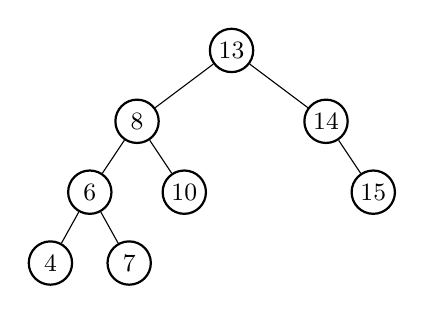
\begin{tikzpicture}[avl,y=0.9cm]
        \node[nd] (n13) at (0,0) {13};
        \node[nd] (n8) at (-1.2,-1) {8};
        \node[nd] (n14) at (1.2,-1) {14};
        \node[nd] (n6) at (-1.8,-2) {6};
        \node[nd] (n10) at (-0.6,-2) {10};
        \node[nd] (n15) at (1.8,-2) {15};
        \node[nd] (n4) at (-2.3,-3) {4};
        \node[nd] (n7) at (-1.3,-3) {7};
        \draw (n13)--(n8) (n13)--(n14) (n8)--(n6) (n8)--(n10)
              (n14)--(n15) (n6)--(n4) (n6)--(n7);
      \end{tikzpicture}\\[4pt]
      {\small 図 3.10(a)\quad AVL木の例}
    \end{column}
  \end{columns}
\end{frame}

% =====================================================
\begin{frame}{AVL木の高さ (1)：節点数が最小の AVL木}
  \textbf{問い}：高さ $h$ の AVL木には，少なくとも何個の節点があるか．
  節点数が最小の木を，$h=0,1,2,3$ について描いてみる．\\[4pt]
  \centering
  \begin{tikzpicture}[avl,y=0.62cm,x=0.8cm]
    \node[hl] at (0,0) {};
    \node at (0,-4.3) {\small $h=0$：1 個};
    \begin{scope}[xshift=2.6cm]
      \node[hl] (a) at (0,0) {}; \node[nd] (b) at (-0.5,-1) {};
      \draw (a)--(b);
      \node at (0,-4.3) {\small $h=1$：2 個};
    \end{scope}
    \begin{scope}[xshift=5.4cm]
      \node[hl] (a) at (0,0) {}; \node[nd] (b) at (-0.8,-1) {};
      \node[nd] (c) at (0.8,-1) {}; \node[nd] (d) at (-1.3,-2) {};
      \draw (a)--(b) (a)--(c) (b)--(d);
      \node at (0,-4.3) {\small $h=2$：4 個};
    \end{scope}
    \begin{scope}[xshift=10.2cm]
      \node[hl] (a) at (0,0) {}; \node[nd] (b) at (-1.5,-1) {};
      \node[nd] (c) at (1.2,-1) {}; \node[nd] (d) at (-2.2,-2) {};
      \node[nd] (e) at (-0.8,-2) {}; \node[nd] (f) at (0.7,-2) {};
      \node[nd] (g) at (-2.7,-3) {};
      \draw (a)--(b) (a)--(c) (b)--(d) (b)--(e) (c)--(f) (d)--(g);
      \node at (-0.2,-4.3) {\small $h=3$：7 個};
    \end{scope}
  \end{tikzpicture}\\[6pt]
  \raggedright
  規則：根の下に，一方は「高さ $h-1$ で節点数最小の木」，もう一方は
  「高さ $h-2$ で節点数最小の木」を置く（差は 1 まで許される）．
\end{frame}

% =====================================================
\begin{frame}{AVL木の高さ (2)：一般の $h$ と漸化式}
  目標：$n$ 節点の任意の AVL木の高さが $O(\log n)$ であることを示す．
  \begin{columns}[T]
    \begin{column}{0.55\textwidth}
      \begin{itemize}
        \item 高さ $h$ の AVL木の節点数は\alert{最大} $2^{h+1}-1$（完全2分木の場合）
        \item 高さ $h$ の AVL木の節点数の\alert{最小値}を $f(h)$ とおく
      \end{itemize}
      \begin{block}{最小の木の構造}
        節点数が最小となるのは左右のバランスが最もくずれている場合：
        根の左部分木の高さが $h-1$，右部分木の高さが $h-2$（その逆でもよい）．
        \[
          f(h) = f(h-1) + f(h-2) + 1
        \]
        {\small 初期条件：$f(0)=1,\ f(1)=2$}
      \end{block}
    \end{column}
    \begin{column}{0.42\textwidth}
      \centering
      \begin{tikzpicture}[avl,y=0.9cm,x=0.9cm]
        \node[nd,hl] (r) at (0,0) {};
        \node[font=\small,accent,right] at (0.35,0) {$+1$（根）};
        % 左部分木：高さ h-1
        \draw (r) -- (-1.3,-1);
        \draw[fill=main!10] (-1.3,-1) -- (-1.9,-3) -- (-0.7,-3) -- cycle;
        \node[font=\scriptsize] at (-1.3,-2.5) {$T_{h-1}$};
        \node[font=\small,main] at (-1.3,-3.4) {$f(h-1)$};
        \draw[<->] (-2.2,-1) -- (-2.2,-3) node[midway,left,font=\scriptsize] {$h-1$};
        % 右部分木：高さ h-2
        \draw (r) -- (1.3,-1);
        \draw[fill=accent!10] (1.3,-1) -- (0.7,-2) -- (1.9,-2) -- cycle;
        \node[font=\scriptsize] at (1.3,-1.65) {$T_{h-2}$};
        \node[font=\small,accent] at (1.3,-2.4) {$f(h-2)$};
        \draw[<->] (2.2,-1) -- (2.2,-2) node[midway,right,font=\scriptsize] {$h-2$};
      \end{tikzpicture}\\[4pt]
      {\small 各部分木もまた節点数最小の\\ AVL木でなければならない}
    \end{column}
  \end{columns}
\end{frame}

% =====================================================
\begin{frame}{AVL木の高さ (3)：漸化式を解く}
  漸化式 $f(h)=f(h-1)+f(h-2)+1$ の両辺に $1$ を足すと
  \[
    \underbrace{f(h)+1}_{F(h)} = \underbrace{\bigl(f(h-1)+1\bigr)}_{F(h-1)}
      + \underbrace{\bigl(f(h-2)+1\bigr)}_{F(h-2)}
  \]
  すなわち $F(h)=f(h)+1$ は「各項 $=$ 前の2項の和」，\alert{フィボナッチ数列}と同じ漸化式．
  \begin{itemize}
    \item \textbf{直観}：$F(h)=F(h-1)+F(h-2)\ge 2F(h-2)$．
          高さが 2 増えるごとに $F(h)$ は\alert{2倍以上}になる $\Rightarrow$ 指数的に増える
    \item これだけで高さが見積もれる．$F(h)\ge 2^{\lfloor h/2\rfloor}F(0\text{ または }1)\ge 2^{\lfloor h/2\rfloor+1}$ で，
          $F(h)=f(h)+1\le n+1$ だから
          \[ h\le 2\log_2(n+1)\quad\Rightarrow\quad h=O(\log n) \]
  \end{itemize}
  より正確な式が欲しければ，初期条件 $F(0)=2,\ F(1)=3$ から一般項が求まる（次ページ）．
\end{frame}

% =====================================================
\begin{frame}{AVL木の高さ (4)：より正確な式（フィボナッチ数列）}
  前ページの $F(h)=f(h)+1$ は，つぎの漸化式をみたす：
  \[
    F(h) = F(h-1) + F(h-2),\qquad F(0)=2,\ F(1)=3
  \]
  これはフィボナッチ (L.\,P.~Fibonacci) 数列で，一般項は
  \[
    F(h) = \frac{\phi_1^{\,h+3}-\phi_2^{\,h+3}}{\sqrt5},\qquad
    \phi_1 = \frac{1+\sqrt5}{2},\quad \phi_2 = \frac{1-\sqrt5}{2}
  \]
  （代入すれば確かめられる）．したがって
  \[
    f(h) = \frac{\phi_1^{\,h+3}-\phi_2^{\,h+3}}{\sqrt5} - 1 \tag{3.2}
  \]
  \begin{alertblock}{結論}
    $f(h) \le n$ を $h$ について解くと，$h = O(\log n)$ をより正確な形で得る（証明は問題 (4)）．
  \end{alertblock}
\end{frame}

% =====================================================
\begin{frame}{AVL木の操作}
  \begin{itemize}
    \item \textbf{MEMBER, MIN}：一般の2分探索木と全く同様に実行すればよい
    \item \textbf{INSERT, DELETE}：前半は一般の場合と同様．
          そのあと AVL木の条件が破れていれば，\alert{回転}で形を直す
    \item 回転は，木の形を変えるが\alert{2分探索木の条件を保つ}操作
  \end{itemize}
\end{frame}

% =====================================================
\begin{frame}{INSERT の考え方 (1)：一直線に傾いた例}
  \centering
  \begin{tikzpicture}[avl,y=0.8cm]
    \node[nd] (a) at (0,0) {3};
    \node[nd] (b) at (-0.8,-1) {2};
    \node[hl] (c) at (-1.6,-2) {1};
    \draw (a)--(b) (b)--(c);
    \node[font=\scriptsize,accent,left] at (-2.0,-2) {挿入};
    \node at (-0.8,-3.1) {\small 3 で傾きすぎ（左が 2 高い）};
    \node at (2.6,-1.2) {\rotarrow};
    \begin{scope}[xshift=5.2cm]
      \node[nd] (a) at (0,0) {2};
      \node[nd] (b) at (-0.9,-1) {1};
      \node[nd] (c) at (0.9,-1) {3};
      \draw (a)--(b) (a)--(c);
      \node at (0,-3.1) {\small 釣り合いが回復};
    \end{scope}
  \end{tikzpicture}\\[8pt]
  \raggedright
  \begin{itemize}
    \item 新しい節点で，ある部分木が1だけ高くなる
    \item 傾いた部分には値が 3 つ（1, 2, 3）しかなく，釣り合う並べ方は\alert{真ん中の値 2 を根にする形}だけ．この組み替えが\alert{回転}
    \item 回転の前後で，左から右へ $1,2,3$ の並びは同じ $\Rightarrow$ 2分探索木の条件は保たれる
  \end{itemize}
\end{frame}

% =====================================================
\begin{frame}{INSERT の考え方 (2)：折れ曲がった例}
  \centering
  \begin{tikzpicture}[avl,y=0.8cm]
    \node[nd] (a) at (0,0) {3};
    \node[nd] (b) at (-0.9,-1) {1};
    \node[hl] (c) at (-0.1,-2) {2};
    \draw (a)--(b) (b)--(c);
    \node[font=\scriptsize,accent,right] at (0.3,-2) {挿入};
    \node at (-0.4,-3.1) {\small 3 で傾きすぎ，ただし左の子 1 は右が高い};
    \node at (3.2,-1.2) {\rotarrow};
    \begin{scope}[xshift=6cm]
      \node[nd] (a) at (0,0) {2};
      \node[nd] (b) at (-0.9,-1) {1};
      \node[nd] (c) at (0.9,-1) {3};
      \draw (a)--(b) (a)--(c);
      \node at (0,-3.1) {\small 釣り合いが回復};
    \end{scope}
  \end{tikzpicture}\\[8pt]
  \raggedright
  \begin{itemize}
    \item 前の例と同じ「傾きすぎ」でも，形が違う：前は左の子の\alert{左}が深く，今回は\alert{右}が深い
    \item 前の例と同じく左の子 1 を根へ持ち上げても直らない（1 を根にしても，3 の左に 2 がぶら下がり，傾きが残る）
          $\Rightarrow$ 3 節点 1, 2, 3 を組み替えて，\alert{2 を根，1 と 3 をその左右の子}にする
    \item 結果はどちらも，真ん中の値 2 が根になる
  \end{itemize}
\end{frame}

% =====================================================
\begin{frame}{INSERT の考え方 (3)：大きな木で下から上へ調べる}
  要素 $2$ を挿入する．新しい節点から根へ向かって，各節点で
  \alert{傾きすぎていないか}を調べる．
  差 $d=$（左の高さ）$-$（右の高さ）とする．
  \begin{columns}[T]
    \begin{column}{0.46\textwidth}
      \centering
      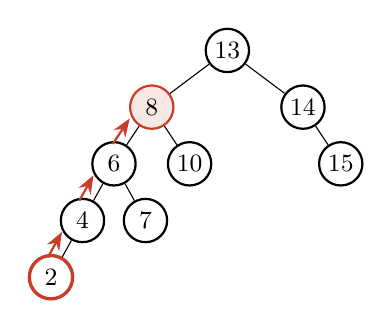
\begin{tikzpicture}[avl,y=0.72cm,x=0.8cm]
        \node[nd] (n13) at (0,0) {13};
        \node[hl] (n8) at (-1.2,-1) {8};
        \node[nd] (n14) at (1.2,-1) {14};
        \node[nd] (n6) at (-1.8,-2) {6};
        \node[nd] (n10) at (-0.6,-2) {10};
        \node[nd] (n15) at (1.8,-2) {15};
        \node[nd] (n4) at (-2.3,-3) {4};
        \node[nd] (n7) at (-1.3,-3) {7};
        \node[nd,draw=accent,very thick] (n2) at (-2.8,-4) {2};
        \draw (n13)--(n8) (n13)--(n14) (n8)--(n6) (n8)--(n10)
              (n14)--(n15) (n6)--(n4) (n6)--(n7) (n4)--(n2);
        \draw[-{Stealth},accent,thick] ($(n2)!0.3!(n4)+(-0.2,0.05)$) -- ($(n2)!0.75!(n4)+(-0.2,0.05)$);
        \draw[-{Stealth},accent,thick] ($(n4)!0.3!(n6)+(-0.2,0.05)$) -- ($(n4)!0.75!(n6)+(-0.2,0.05)$);
        \draw[-{Stealth},accent,thick] ($(n6)!0.3!(n8)+(-0.2,0.05)$) -- ($(n6)!0.75!(n8)+(-0.2,0.05)$);
      \end{tikzpicture}
    \end{column}
    \begin{column}{0.52\textwidth}
      \renewcommand{\arraystretch}{1.35}
      \small
      \begin{tabular}{c|cc|l}
        節点 & 前 $d$ & 後 $d$ & 判断 \\\hline
        $4$ & $0$ & $+1$ & 高さ増加 $\Rightarrow$ 上へ \\
        $6$ & $0$ & $+1$ & 高さ増加 $\Rightarrow$ 上へ \\
        $8$ & $+1$ & \alert{$+2$} & \alert{傾きすぎ $\Rightarrow$ 回転}
      \end{tabular}\\[2pt]
      {\scriptsize 前／後：挿入前／後の $d$}
    \end{column}
  \end{columns}
  \vspace{4pt}
  各節点で，新しい差は「\alert{挿入前の差}」と「左が高くなった」ことだけから決まる．
\end{frame}

% =====================================================
\begin{frame}{INSERT の考え方 (4)：大きな木での回転}
  \centering
  \begin{tikzpicture}[avl,y=0.6cm,x=0.85cm]
    \begin{scope}
      \node[nd] (n13) at (0,0) {13};
      \node[hl,nm=u] (n8) at (-1.2,-1) {8};
      \node[nd] (n14) at (1.2,-1) {14};
      \node[hl,nm=v] (n6) at (-1.8,-2) {6};
      \node[nd,fill=orange!35] (n10) at (-0.6,-2) {10};
      \node[nd] (n15) at (1.8,-2) {15};
      \node[nd,fill=blue!22] (n4) at (-2.3,-3) {4};
      \node[nd,fill=green!30] (n7) at (-1.3,-3) {7};
      \node[nd,fill=blue!22] (n2) at (-2.8,-4) {2};
      \draw (n13)--(n8) (n13)--(n14) (n8)--(n6) (n8)--(n10)
            (n14)--(n15) (n6)--(n4) (n6)--(n7) (n4)--(n2);
      \node at (0,-5.0) {\small 回転前（8 で $d=+2$）};
    \end{scope}
    \node at (3.4,-2) {\rotarrow};
    \begin{scope}[xshift=7.4cm]
      \node[nd] (n13) at (0,0) {13};
      \node[hl,nm=v] (n6) at (-1.2,-1) {6};
      \node[nd] (n14) at (1.2,-1) {14};
      \node[nd,fill=blue!22] (n4) at (-1.9,-2) {4};
      \node[hl,nm=u] (n8) at (-0.5,-2) {8};
      \node[nd] (n15) at (1.8,-2) {15};
      \node[nd,fill=blue!22] (n2) at (-2.3,-3) {2};
      \node[nd,fill=green!30] (n7) at (-0.9,-3) {7};
      \node[nd,fill=orange!35] (n10) at (-0.1,-3) {10};
      \draw (n13)--(n6) (n13)--(n14) (n6)--(n4) (n6)--(n8)
            (n4)--(n2) (n8)--(n7) (n8)--(n10) (n14)--(n15);
      \node at (0,-5.0) {\small 回転後};
    \end{scope}
  \end{tikzpicture}\\[2pt]
  \raggedright\small
  $u=8$（傾いた節点），$v=6$（その左の子）．
  \colorbox{blue!22}{$\alpha=\{4,2\}$}，\colorbox{green!30}{$\beta=\{7\}$}，\colorbox{orange!35}{$\gamma=\{10\}$}．
  \begin{enumerate}
    \item $v$ を $u$ の位置へ持ち上げる（13 の左の子が 6 になる）
    \item $u$ を $v$ の右の子にする
    \item $\beta$ を $v$ の右から $u$ の左へつけかえる．$\alpha$ は $v$ の左，$\gamma$ は $u$ の右のまま
  \end{enumerate}
  2分探索木の条件は保たれる（左から右へ $\alpha,6,\beta,8,\gamma$ の並びは同じ）．6 の左右の高さはともに 1 で釣り合い，
  部分木の高さは挿入前の 8 と同じ（2）$\Rightarrow$ 上の節点は変わらず，終了．
\end{frame}

% =====================================================
\begin{frame}{INSERT の考え方 (5)：高さが変わらない例}
  \centering
  \begin{tikzpicture}[avl,y=0.7cm,x=0.85cm]
    \begin{scope}
      \node[nd] (a) at (0,0) {5}; \node[nd] (b) at (-1.0,-1) {2};
      \node[nd] (c) at (1.0,-1) {8}; \node[nd] (d) at (-0.4,-2) {3};
      \draw (a)--(b) (a)--(c) (b)--(d);
      \node at (0,-3.2) {\small 挿入前：2 の右が高い（$d=-1$）};
    \end{scope}
    \node at (3.2,-1.2) {\insarrow};
    \begin{scope}[xshift=6.3cm]
      \node[nd] (a) at (0,0) {5}; \node[nd] (b) at (-1.0,-1) {2};
      \node[nd] (c) at (1.0,-1) {8}; \node[nd] (d) at (-0.4,-2) {3};
      \node[hl] (e) at (-1.6,-2) {1};
      \draw (a)--(b) (a)--(c) (b)--(d) (b)--(e);
      \node at (0,-3.2) {\small 1 を挿入：2 は釣り合う（$d=0$）};
    \end{scope}
  \end{tikzpicture}\\[4pt]
  \raggedright\small
  \begin{enumerate}
    \item 1 を挿入すると 2 の左が高くなるが，もともと右が高かったので，左右の高さが等しくなるだけ．傾きすぎない．
    \item 2 を根とする部分木の高さは $1$ のまま $\Rightarrow$ 5 から上の節点の左右の高さは何も変わらない．
    \item よって，この場合は回転も，それより上の調べも要らず，修正は\alert{ここで終了}．
  \end{enumerate}
\end{frame}

% =====================================================
\begin{frame}{INSERT の考え方 (6)：回転すべきかの判断}
  左の部分木が1高くなって上ってきたとき，節点 $y$ では
  \begin{center}
    \renewcommand{\arraystretch}{1.3}
    \begin{tabular}{c|c|l}
      挿入前の $d$ & 挿入後の $d$ & 判断 \\\hline
      $-1$ & $0$ & 高さは変わらない（例 (5)）$\Rightarrow$ 終了 \\
      $0$ & $+1$ & 高さが増えた $\Rightarrow$ さらに上へ \\
      $+1$ & $+2$ & 傾きすぎ $\Rightarrow$ \alert{回転}
    \end{tabular}
  \end{center}
  \begin{itemize}
    \item 判断に必要なのは\alert{挿入前の差 $d$ だけ}．部分木の高さそのものは要らない
    \item どの形に組み替えるか（図 3.11 の (a) か (b) か）は，傾いた側の子がどちらに深いか（その子の差の符号）で決まる
  \end{itemize}
  \begin{block}{気づき}
    AVL木では $d\in\{-1,0,+1\}$ の\alert{3通りしかない}．
    $\Rightarrow$ 各節点に，どちらが高いか（3状態）だけを記憶すれば十分．
  \end{block}
\end{frame}

% =====================================================
\begin{frame}{平衡状態 $s(y)$}
  \alert{どちら側が高いか}を各節点に記憶する：
  \begin{columns}[T]
    \begin{column}{0.6\textwidth}
      \begin{block}{平衡状態 $s(y)$}
        節点 $y$ の左部分木 $T_L$，右部分木 $T_R$ に対し
        \[
          s(y) =
          \begin{cases}
            L, & |T_L| > |T_R| \quad(\text{差 }+1)\\
            R, & |T_L| < |T_R| \quad(\text{差 }-1)\\
            E, & |T_L| = |T_R| \quad(\text{差 }0)
          \end{cases}
        \]
        {\small $|T|$ は $T$ の高さ}
      \end{block}
      \begin{itemize}
        \item 各節点に $s(y)\in\{L,R,E\}$ を記憶する
        \item 挿入・除去のたびに $s(y)$ を更新し，差が $\pm2$ になりそうなときだけ修正すればよい
      \end{itemize}
    \end{column}
    \begin{column}{0.36\textwidth}
      \centering
      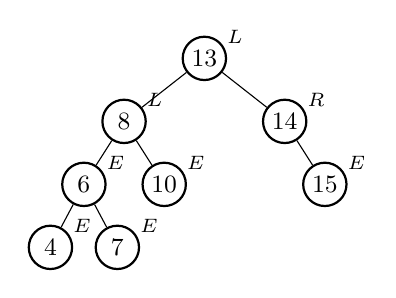
\begin{tikzpicture}[avl,y=0.8cm,x=0.85cm]
        \node[nd,bal=L] (n13) at (0,0) {13};
        \node[nd,bal=L] (n8) at (-1.2,-1) {8};
        \node[nd,bal=R] (n14) at (1.2,-1) {14};
        \node[nd,bal=E] (n6) at (-1.8,-2) {6};
        \node[nd,bal=E] (n10) at (-0.6,-2) {10};
        \node[nd,bal=E] (n15) at (1.8,-2) {15};
        \node[nd,bal=E] (n4) at (-2.3,-3) {4};
        \node[nd,bal=E] (n7) at (-1.3,-3) {7};
        \draw (n13)--(n8) (n13)--(n14) (n8)--(n6) (n8)--(n10)
              (n14)--(n15) (n6)--(n4) (n6)--(n7);
      \end{tikzpicture}\\[2pt]
      {\small 図 3.10(a)\quad $s(y)$ つきの AVL木}
    \end{column}
  \end{columns}
\end{frame}

% =====================================================
\begin{frame}{図 3.11(a)　INSERT の回転（一般）：$s(v)=L$ の場合}
  \centering
  \begin{tikzpicture}[avl]
    % 回転前
    \node[nd,bal=L] (u) at (0,0) {$u$};
    \node[hl,bal=L] (v) at (-1.1,-1) {$v$};
    \draw (u)--(v);
    \sub{v}{-1.6}{-2}{-4}{\alpha} \ext{-1.6}{-4}{1}
    \sub{v}{-0.6}{-2}{-4}{\beta}
    \sub{u}{1}{-1}{-3}{\gamma}
    \node[font=\scriptsize,accent,align=right,left] at (-1.45,-0.6) {高さが\\1増加};
    % 矢印
    \node at (2.4,-2) {\rotarrow};
    % 回転後
    \begin{scope}[xshift=4.8cm]
      \node[nd,bal=E] (v2) at (0,0) {$v$};
      \node[nd,bal=E] (u2) at (1,-1) {$u$};
      \draw (v2)--(u2);
      \sub{v2}{-1}{-1}{-3}{\alpha} \ext{-1}{-3}{1}
      \sub{u2}{0.5}{-2}{-4}{\beta}
      \sub{u2}{1.5}{-2}{-4}{\gamma}
    \end{scope}
  \end{tikzpicture}\\[6pt]
  \small 破線：挿入により $\alpha$ の高さが1増えた部分．\\
  2分探索木の条件は保たれる（左から右へ $\alpha, v, \beta, u, \gamma$ の並びは同じ）．\\
  回転後：$s(v)=s(u)=E$，部分木の高さは挿入前と同じ．
\end{frame}

% =====================================================
\begin{frame}{図 3.11(b)　INSERT の回転（一般）：$s(v)=R$ の場合}
  \centering
  \begin{tikzpicture}[avl]
    % 回転前
    \node[nd,bal=L] (u) at (0,0) {$u$};
    \node[hl,bal=R] (v) at (-1.2,-1) {$v$};
    \node[nd,bal=L] (w) at (-0.5,-2) {$w$};
    \draw (u)--(v) (v)--(w);
    \sub{v}{-1.8}{-2}{-5}{\alpha}
    \sub{w}{-0.9}{-3}{-5}{\beta} \ext{-0.9}{-5}{1}
    \sub{w}{-0.1}{-3}{-5}{\gamma}
    \sub{u}{1}{-1}{-4}{\delta}
    \node[font=\scriptsize,accent,align=right,left] at (-1.55,-0.6) {高さが\\1増加};
    \node at (2.3,-2.5) {\rotarrow};
    % 回転後
    \begin{scope}[xshift=4.8cm]
      \node[nd,bal=E] (w2) at (0,0) {$w$};
      \node[nd,bal=E] (v2) at (-1,-1) {$v$};
      \node[nd,bal=R] (u2) at (1,-1) {$u$};
      \draw (w2)--(v2) (w2)--(u2);
      \sub{v2}{-1.5}{-2}{-5}{\alpha}
      \sub{v2}{-0.5}{-2}{-4}{\beta} \ext{-0.5}{-4}{1}
      \sub{u2}{0.5}{-2}{-4}{\gamma}
      \sub{u2}{1.5}{-2}{-5}{\delta}
    \end{scope}
  \end{tikzpicture}\\[4pt]
  \small 図は $s(w)=L$（$\beta$ 側が伸びた）場合．$s(w)=R$ の場合も同様（問題 3.5）．\\
  2分探索木の条件は保たれる（左から右へ $\alpha, v, \beta, w, \gamma, u, \delta$ の並びは同じ）．回転後の部分木の高さは挿入前と同じ．
\end{frame}

% =====================================================
\begin{frame}{INSERT$(x,A)$ の修正手順}
  \begin{itemize}
    \item $x$ を新しい位置に挿入するまでは一般の場合と同様
    \item その結果，部分木によってはその高さが1増加 $\Rightarrow$ $x$ から根へ向かって修正
    \item 左の子 $v$ からその親 $u$ へのぼってきたとする（右の子からの場合は，左右を入れ替えて同様に考える）．
          すなわち $v$ を根とする部分木の高さが1増えた状態（そうでなければ修正不要）
  \end{itemize}
  \begin{block}{INSERT 実行前の $s(u)$ による場合分け}
    \begin{enumerate}
      \item $s(u)=R$：$s(u)=E$ に変わる．$u$ を根とする部分木の高さは不変 $\Rightarrow$ \alert{終了}
      \item $s(u)=E$：$s(u)=L$ に変わる．$u$ の部分木は AVL木だが高さが1増加
            $\Rightarrow$ $u$ の親へさかのぼり\alert{続行}（$u$ が根なら終了）
      \item $s(u)=L$：$u$ で AVL木の条件が破れる．$s(v)$ に応じて
            図 3.11(a)，(b) のような\alert{回転}を施す．回転後の部分木は AVL木で，
            高さは修正前と等しい $\Rightarrow$ \alert{終了}
    \end{enumerate}
  \end{block}
\end{frame}

% =====================================================
\begin{frame}{証明 (1)：INSERT の手順を再帰の形で述べる}
  \footnotesize
  ここまでで INSERT の修正手順を述べた．以降では，この手順を実行しても AVL木が保たれることを示す．\\[2pt]
  INSERT は再帰的に説明できる．根が $u$ の木に $x$ を挿入するには，$x$ が小さければ左部分木に，そうでなければ右部分木に挿入する（以降は左の場合を述べる．右の場合は，左右を入れ替えて同様に行う）．
  \begin{itemize}
    \item 木が空なら，$x$ だけの葉にする．
    \item そうでなければ，まず左部分木に $x$ を挿入する（より小さい木での同じ問題）．そのあと，左部分木の高さを見る：
      \begin{itemize}
        \item 高くなっていなければ，$u$ では何もしない．
        \item 1高くなっていれば，挿入前の $s(u)$ に応じて：
          $R$ なら $E$ にする（$u$ の高さは不変）．
          $E$ なら $L$ にする（$u$ の高さは1増える）．
          $L$ なら図 3.11(a)，(b) のような回転を施す．
      \end{itemize}
  \end{itemize}
\end{frame}

% =====================================================
\begin{frame}{証明 (2)：INSERT について示すこと}
  \footnotesize
  \begin{alertblock}{示すこと}
    各節点 $y$ について，$d(y)=$（左部分木の高さ）$-$（右部分木の高さ）とする．
    すべての節点 $y$ で $|d(y)|\le1$ であり，保存された $s(y)$ が $d(y)$ に対応する値（$d=+1,0,-1$ に対して $L,E,R$）である2分探索木に，この手順で $x$ を挿入する．
    このとき，木全体と，それに含まれる\alert{どの部分木}についても，
    \begin{enumerate}
      \item 2分探索木であり，$x$ を含む．
      \item どの節点 $y$ でも $|d(y)|\le1$ で，$s(y)$ は $d(y)$ に対応する値である（\alert{AVL木のまま}）．
      \item 高さは変わらないか，ちょうど1増える．
    \end{enumerate}
  \end{alertblock}
  \vspace{4pt}
  (2) は「どの部分木も AVL木のまま」を，(3) は「その部分木より上の節点に影響するかどうか」を表す．
\end{frame}

% =====================================================
\begin{frame}{証明 (3)：使う事実}
  \footnotesize
  挿入前に $s(u)=L$ だった節点 $u$ で，挿入によって左部分木が1高くなったとする（$u$ は傾きすぎ）．
  挿入後の左部分木の根を $v$ とする．
  つぎの事実は，図 3.11 とその説明，および問題 3.5（その解答を含む）から成り立つものとして，そのまま使う．
  \begin{block}{事実}
    \begin{itemize}
      \item[(F1)] 挿入前に $s(u)=L$ であり，かつ挿入によって $u$ の左部分木（根 $v$）の高さが1増えたならば，
        挿入後 $s(v)=L$ または $s(v)=R$ であり，$s(v)=E$ とはならない．（問題 3.5(iii)）
      \item[(F2)] $s(v)=L$ のときは図 3.11(a)，$s(v)=R$ のときは図 3.11(b) の回転を施す．
        図 3.11(b) は $s(w)=L$ の場合の図である．$s(w)=R$ の場合を含め，
        AVL木の条件を回復する回転が存在する．（問題 3.5(i)）
      \item[(F3)] 回転後の部分木は，(a)，および (b) の $s(w)=L$，$s(w)=R$ のいずれの場合も AVL木の条件をみたす．（問題 3.5(ii)）
    \end{itemize}
  \end{block}
  \begin{block}{図 3.11 から読み取れること}
    回転後の部分木の高さは，挿入前の $u$ の部分木の高さに等しい．
    また，回転後の $s(u),s(v),s(w)$ は，図の右側のように定める．
  \end{block}
\end{frame}

% =====================================================
\begin{frame}{証明 (4)：空の木，左部分木が高くならない場合}
  \footnotesize
  \textbf{空の木}：結果は葉ひとつ．釣り合っていて状態は $E$．高さは $-1$ から $0$ になり，ちょうど1増える．\\[2pt]
  \textbf{空でない木}：挿入前の左右の部分木の高さを $a,\ b$ とする（$|a-b|\le1$）．右部分木は変わらず，もともと問題ない．
  左部分木への挿入は，より小さい木への同じ挿入なので，新しい左部分木は (1)〜(3) をみたす．2分探索木であることは，回転が部分木を組み替えるだけで
  左から右への並びを変えないことから，どの場合も成り立つ．\\[2pt]
  \textbf{左部分木の高さが増えなかった}：$u$ での差は変わらないので，$u$ は釣り合い，$s(u)$ も正しいまま．木の高さも変わらない．
  \begin{center}
  \begin{tikzpicture}[avl,y=0.4cm]
\node[font=\small\bfseries,main] at (1.6,1.9) {空の木};
\begin{scope}[xshift=0cm]
\node[font=\large] at (0,-1) {$\emptyset$};
\node[font=\scriptsize,align=center,anchor=north] at (0,-4.7) {空の木\\高さ $-1$};
\end{scope}
\node at (1.6,-1.5) {\insarrow};
\begin{scope}[xshift=3.2cm]
\node[hl,label={[font=\scriptsize\itshape,inner sep=1pt]30:$E$}] (x0) at (0,-1) {$x$};
\node[font=\scriptsize,align=center,anchor=north] at (0,-4.7) {葉ひとつ\\高さ $0$（1増える）};
\end{scope}
\node[font=\small\bfseries,main] at (8.8,1.9) {左部分木の高さが増えなかった};
\begin{scope}[xshift=7.2cm]
\node[nd,label={[font=\scriptsize\itshape,inner sep=1pt]30:$s$}] (a1) at (0,0) {$u$};
\draw (a1) -- (-0.6,-1); \fill (-0.6,-1) circle (1.2pt);
\draw[fill=white] (-0.6,-1) -- (-0.93,-3) -- (-0.27,-3) -- cycle;
\node[font=\scriptsize,below,inner sep=1pt] at (-0.6,-3) {$a$};
\draw (a1) -- (0.6,-1); \fill (0.6,-1) circle (1.2pt);
\draw[fill=white] (0.6,-1) -- (0.27,-3) -- (0.93,-3) -- cycle;
\node[font=\scriptsize,below,inner sep=1pt] at (0.6,-3) {$b$};
\node[font=\scriptsize,align=center,anchor=north] at (0,-4.7) {挿入前};
\end{scope}
\node at (8.8,-1.5) {\insarrow};
\begin{scope}[xshift=10.4cm]
\node[nd,label={[font=\scriptsize\itshape,inner sep=1pt]30:$s$}] (a2) at (0,0) {$u$};
\draw (a2) -- (-0.6,-1); \fill (-0.6,-1) circle (1.2pt);
\draw[fill=accent!20] (-0.6,-1) -- (-0.93,-3) -- (-0.27,-3) -- cycle;
\node[font=\scriptsize,below,inner sep=1pt] at (-0.6,-3) {$a$};
\draw (a2) -- (0.6,-1); \fill (0.6,-1) circle (1.2pt);
\draw[fill=white] (0.6,-1) -- (0.27,-3) -- (0.93,-3) -- cycle;
\node[font=\scriptsize,below,inner sep=1pt] at (0.6,-3) {$b$};
\node[font=\scriptsize,align=center,anchor=north] at (0,-4.7) {$u$ での差も $s(u)$ もそのまま\\高さ不変};
\end{scope}
  \end{tikzpicture}
  \end{center}
  \vspace{-6pt}\scriptsize 三角形の下は部分木の高さ，節点の肩は状態 $s$．色付きは挿入で高さが変わった部分木．
\end{frame}

% =====================================================
\begin{frame}{証明 (5)：左部分木が1高くなり，挿入前 $s(u)=R$ または $E$}
  \footnotesize
  左部分木の新しい高さは $a+1$．
  \begin{itemize}
    \item \textbf{挿入前 $s(u)=R$}（$b=a+1$）：左右の高さが等しくなるので $s(u)=E$ が正しい．高さは $b+1$ で挿入前と同じ．
    \item \textbf{挿入前 $s(u)=E$}（$b=a$）：左が1高くなるので $s(u)=L$ が正しく，釣り合ったまま．高さは1増える．
  \end{itemize}
  \begin{center}
  \begin{tikzpicture}[avl,y=0.4cm]
\node[font=\small\bfseries,main] at (1.6,1.9) {挿入前 $s(u)=R$（$b=a+1$）};
\begin{scope}[xshift=0cm]
\node[nd,label={[font=\scriptsize\itshape,inner sep=1pt]30:$R$}] (r1) at (0,0) {$u$};
\draw (r1) -- (-0.6,-1); \fill (-0.6,-1) circle (1.2pt);
\draw[fill=white] (-0.6,-1) -- (-0.93,-3) -- (-0.27,-3) -- cycle;
\node[font=\scriptsize,below,inner sep=1pt] at (-0.6,-3) {$a$};
\draw (r1) -- (0.6,-1); \fill (0.6,-1) circle (1.2pt);
\draw[fill=white] (0.6,-1) -- (0.27,-4) -- (0.93,-4) -- cycle;
\node[font=\scriptsize,below,inner sep=1pt] at (0.6,-4) {$a{+}1$};
\node[font=\scriptsize,align=center,anchor=north] at (0,-4.7) {挿入前\\高さ $a+2$};
\end{scope}
\node at (1.6,-1.5) {\insarrow};
\begin{scope}[xshift=3.2cm]
\node[nd,label={[font=\scriptsize\itshape,inner sep=1pt]30:$E$}] (r2) at (0,0) {$u$};
\draw (r2) -- (-0.6,-1); \fill (-0.6,-1) circle (1.2pt);
\draw[fill=accent!20] (-0.6,-1) -- (-0.93,-4) -- (-0.27,-4) -- cycle;
\node[font=\scriptsize,below,inner sep=1pt] at (-0.6,-4) {$a{+}1$};
\draw (r2) -- (0.6,-1); \fill (0.6,-1) circle (1.2pt);
\draw[fill=white] (0.6,-1) -- (0.27,-4) -- (0.93,-4) -- cycle;
\node[font=\scriptsize,below,inner sep=1pt] at (0.6,-4) {$a{+}1$};
\node[font=\scriptsize,align=center,anchor=north] at (0,-4.7) {左右が等しい：$s(u)=E$\\高さ $a+2$（不変）};
\end{scope}
\node[font=\small\bfseries,main] at (8.8,1.9) {挿入前 $s(u)=E$（$b=a$）};
\begin{scope}[xshift=7.2cm]
\node[nd,label={[font=\scriptsize\itshape,inner sep=1pt]30:$E$}] (e1) at (0,0) {$u$};
\draw (e1) -- (-0.6,-1); \fill (-0.6,-1) circle (1.2pt);
\draw[fill=white] (-0.6,-1) -- (-0.93,-3) -- (-0.27,-3) -- cycle;
\node[font=\scriptsize,below,inner sep=1pt] at (-0.6,-3) {$a$};
\draw (e1) -- (0.6,-1); \fill (0.6,-1) circle (1.2pt);
\draw[fill=white] (0.6,-1) -- (0.27,-3) -- (0.93,-3) -- cycle;
\node[font=\scriptsize,below,inner sep=1pt] at (0.6,-3) {$a$};
\node[font=\scriptsize,align=center,anchor=north] at (0,-4.7) {挿入前\\高さ $a+1$};
\end{scope}
\node at (8.8,-1.5) {\insarrow};
\begin{scope}[xshift=10.4cm]
\node[nd,label={[font=\scriptsize\itshape,inner sep=1pt]30:$L$}] (e2) at (0,0) {$u$};
\draw (e2) -- (-0.6,-1); \fill (-0.6,-1) circle (1.2pt);
\draw[fill=accent!20] (-0.6,-1) -- (-0.93,-4) -- (-0.27,-4) -- cycle;
\node[font=\scriptsize,below,inner sep=1pt] at (-0.6,-4) {$a{+}1$};
\draw (e2) -- (0.6,-1); \fill (0.6,-1) circle (1.2pt);
\draw[fill=white] (0.6,-1) -- (0.27,-3) -- (0.93,-3) -- cycle;
\node[font=\scriptsize,below,inner sep=1pt] at (0.6,-3) {$a$};
\node[font=\scriptsize,align=center,anchor=north] at (0,-4.7) {左が1高い：$s(u)=L$\\高さ $a+2$（1増える）};
\end{scope}
  \end{tikzpicture}
  \end{center}
  \vspace{-6pt}\scriptsize 三角形の下は部分木の高さ，節点の肩は状態 $s$．色付きは挿入で高さが変わった部分木．
\end{frame}

% =====================================================
\begin{frame}{証明 (6)：挿入前 $s(u)=L$，$s(v)=L$ の場合（図 3.11(a)）}
  \footnotesize
  左部分木の高さが1増え，挿入前 $s(u)=L$（$a=b+1$）のとき，左が右より2高くなるので，回転する．
  (F1)(F2) より，AVL木の条件を回復する回転が存在するので，それを施す．
  (F3) より，回転後の部分木は AVL木の条件をみたす．回転後の $s$ は，回転後の形に合わせて定める．
  また，回転後の部分木の高さは挿入前と同じである（図 3.11）．その他の部分木は変化せず，もともと問題ない．\\[2pt]
  下図は $s(v)=L$ で，図 3.11(a) の回転を施す場合．
  \begin{center}
  \begin{tikzpicture}[avl,y=0.4cm]
\begin{scope}[xshift=0.0cm]
\node[nd,label={[font=\scriptsize\itshape,inner sep=1pt]30:$L$}] (u) at (0,0) {$u$};
\node[nd,label={[font=\scriptsize\itshape,inner sep=1pt]150:$E$}] (v) at (-0.9,-1) {$v$};
\draw (u)--(v);
\draw (v) -- (-1.4,-2); \fill (-1.4,-2) circle (1.2pt);
\draw[fill=white] (-1.4,-2) -- (-1.73,-4) -- (-1.07,-4) -- cycle;
\node[font=\scriptsize,below,inner sep=1pt] at (-1.4,-4) {$k$};
\node[font=\scriptsize] at (-1.4,-3.45) {$\alpha$};
\draw (v) -- (-0.4,-2); \fill (-0.4,-2) circle (1.2pt);
\draw[fill=white] (-0.4,-2) -- (-0.73,-4) -- (-0.07,-4) -- cycle;
\node[font=\scriptsize,below,inner sep=1pt] at (-0.4,-4) {$k$};
\node[font=\scriptsize] at (-0.4,-3.45) {$\beta$};
\draw (u) -- (0.9,-1); \fill (0.9,-1) circle (1.2pt);
\draw[fill=white] (0.9,-1) -- (0.57,-3) -- (1.23,-3) -- cycle;
\node[font=\scriptsize,below,inner sep=1pt] at (0.9,-3) {$k$};
\node[font=\scriptsize] at (0.9,-2.45) {$\gamma$};
\node[font=\scriptsize,align=center,anchor=north] at (0,-6.3) {挿入前\\高さ $k+2$};
\end{scope}
\node at (2.3,-2) {\insarrow};
\begin{scope}[xshift=4.6cm]
\node[nd,label={[font=\scriptsize\itshape,inner sep=1pt]30:$L$}] (u) at (0,0) {$u$};
\node[hl,label={[font=\scriptsize\itshape,inner sep=1pt]150:$L$}] (v) at (-0.9,-1) {$v$};
\draw (u)--(v);
\draw (v) -- (-1.4,-2); \fill (-1.4,-2) circle (1.2pt);
\draw[fill=accent!20] (-1.4,-2) -- (-1.73,-5) -- (-1.07,-5) -- cycle;
\node[font=\scriptsize,below,inner sep=1pt] at (-1.4,-5) {$k{+}1$};
\node[font=\scriptsize] at (-1.4,-4.45) {$\alpha$};
\draw (v) -- (-0.4,-2); \fill (-0.4,-2) circle (1.2pt);
\draw[fill=white] (-0.4,-2) -- (-0.73,-4) -- (-0.07,-4) -- cycle;
\node[font=\scriptsize,below,inner sep=1pt] at (-0.4,-4) {$k$};
\node[font=\scriptsize] at (-0.4,-3.45) {$\beta$};
\draw (u) -- (0.9,-1); \fill (0.9,-1) circle (1.2pt);
\draw[fill=white] (0.9,-1) -- (0.57,-3) -- (1.23,-3) -- cycle;
\node[font=\scriptsize,below,inner sep=1pt] at (0.9,-3) {$k$};
\node[font=\scriptsize] at (0.9,-2.45) {$\gamma$};
\node[font=\scriptsize,align=center,anchor=north] at (0,-6.3) {$\alpha$ に挿入：$\alpha$ が $k+1$\\$u$ で左が2高い};
\end{scope}
\node at (6.8999999999999995,-2) {\rotarrow};
\begin{scope}[xshift=9.2cm]
\node[nd,label={[font=\scriptsize\itshape,inner sep=1pt]30:$E$}] (v) at (0,0) {$v$};
\node[nd,label={[font=\scriptsize\itshape,inner sep=1pt]30:$E$}] (u) at (0.9,-1) {$u$};
\draw (v)--(u);
\draw (v) -- (-0.9,-1); \fill (-0.9,-1) circle (1.2pt);
\draw[fill=accent!20] (-0.9,-1) -- (-1.23,-4) -- (-0.57,-4) -- cycle;
\node[font=\scriptsize,below,inner sep=1pt] at (-0.9,-4) {$k{+}1$};
\node[font=\scriptsize] at (-0.9,-3.45) {$\alpha$};
\draw (u) -- (0.4,-2); \fill (0.4,-2) circle (1.2pt);
\draw[fill=white] (0.4,-2) -- (0.07,-4) -- (0.73,-4) -- cycle;
\node[font=\scriptsize,below,inner sep=1pt] at (0.4,-4) {$k$};
\node[font=\scriptsize] at (0.4,-3.45) {$\beta$};
\draw (u) -- (1.4,-2); \fill (1.4,-2) circle (1.2pt);
\draw[fill=white] (1.4,-2) -- (1.07,-4) -- (1.73,-4) -- cycle;
\node[font=\scriptsize,below,inner sep=1pt] at (1.4,-4) {$k$};
\node[font=\scriptsize] at (1.4,-3.45) {$\gamma$};
\node[font=\scriptsize,align=center,anchor=north] at (0,-6.3) {回転後：$s(v)=s(u)=E$\\高さ $k+2$（挿入前と同じ）};
\end{scope}
  \end{tikzpicture}
  \end{center}
  \vspace{-6pt}\scriptsize 三角形の下は部分木の高さ，節点の肩は状態 $s$．色付きは挿入で高さが変わった部分木．$s(u)$ は挿入前の値．
\end{frame}

% =====================================================
\begin{frame}{証明 (7)：挿入前 $s(u)=L$，$s(v)=R$ の場合（図 3.11(b)）}
  \footnotesize
  (F1) より $s(v)$ は $L$ か $R$．$s(v)=R$ のときは，(F2) より図 3.11(b) の回転を施す．
  (F3) より回転後の部分木は AVL木の条件をみたし，高さは挿入前と同じである（図 3.11）．\\[2pt]
  下図は $s(w)=L$ の場合（図 3.11(b)）．
  \begin{center}
  \begin{tikzpicture}[avl,y=0.4cm]
\begin{scope}[xshift=0.0cm]
\node[nd,label={[font=\scriptsize\itshape,inner sep=1pt]30:$L$}] (u) at (0,0) {$u$};
\node[nd,label={[font=\scriptsize\itshape,inner sep=1pt]150:$E$}] (v) at (-1.0,-1) {$v$};
\node[nd,label={[font=\scriptsize\itshape,inner sep=1pt]30:$E$}] (w) at (-0.4,-2) {$w$};
\draw (u)--(v);
\draw (v)--(w);
\draw (v) -- (-1.6,-2); \fill (-1.6,-2) circle (1.2pt);
\draw[fill=white] (-1.6,-2) -- (-1.93,-4) -- (-1.27,-4) -- cycle;
\node[font=\scriptsize,below,inner sep=1pt] at (-1.6,-4) {$k$};
\node[font=\scriptsize] at (-1.6,-3.45) {$\alpha$};
\draw (w) -- (-0.8,-3); \fill (-0.8,-3) circle (1.2pt);
\draw[fill=white] (-0.8,-3) -- (-1.13,-4) -- (-0.47,-4) -- cycle;
\node[font=\scriptsize,below,inner sep=1pt] at (-0.8,-4) {$k{-}1$};
\draw (w) -- (0.0,-3); \fill (0.0,-3) circle (1.2pt);
\draw[fill=white] (0.0,-3) -- (-0.33,-4) -- (0.33,-4) -- cycle;
\node[font=\scriptsize,below,inner sep=1pt] at (0.0,-4) {$k{-}1$};
\draw (u) -- (1.0,-1); \fill (1.0,-1) circle (1.2pt);
\draw[fill=white] (1.0,-1) -- (0.67,-3) -- (1.33,-3) -- cycle;
\node[font=\scriptsize,below,inner sep=1pt] at (1.0,-3) {$k$};
\node[font=\scriptsize] at (1.0,-2.45) {$\delta$};
\node[font=\scriptsize,align=center,anchor=north] at (0,-6.3) {挿入前\\高さ $k+2$};
\end{scope}
\node at (2.3,-2) {\insarrow};
\begin{scope}[xshift=4.6cm]
\node[nd,label={[font=\scriptsize\itshape,inner sep=1pt]30:$L$}] (u) at (0,0) {$u$};
\node[hl,label={[font=\scriptsize\itshape,inner sep=1pt]150:$R$}] (v) at (-1.0,-1) {$v$};
\node[nd,label={[font=\scriptsize\itshape,inner sep=1pt]30:$L$}] (w) at (-0.4,-2) {$w$};
\draw (u)--(v);
\draw (v)--(w);
\draw (v) -- (-1.6,-2); \fill (-1.6,-2) circle (1.2pt);
\draw[fill=white] (-1.6,-2) -- (-1.93,-4) -- (-1.27,-4) -- cycle;
\node[font=\scriptsize,below,inner sep=1pt] at (-1.6,-4) {$k$};
\node[font=\scriptsize] at (-1.6,-3.45) {$\alpha$};
\draw (w) -- (-0.8,-3); \fill (-0.8,-3) circle (1.2pt);
\draw[fill=accent!20] (-0.8,-3) -- (-1.13,-5) -- (-0.47,-5) -- cycle;
\node[font=\scriptsize,below,inner sep=1pt] at (-0.8,-5) {$k$};
\node[font=\scriptsize] at (-0.8,-4.45) {$\beta$};
\draw (w) -- (0.0,-3); \fill (0.0,-3) circle (1.2pt);
\draw[fill=white] (0.0,-3) -- (-0.33,-4) -- (0.33,-4) -- cycle;
\node[font=\scriptsize,below,inner sep=1pt] at (0.0,-4) {$k{-}1$};
\draw (u) -- (1.0,-1); \fill (1.0,-1) circle (1.2pt);
\draw[fill=white] (1.0,-1) -- (0.67,-3) -- (1.33,-3) -- cycle;
\node[font=\scriptsize,below,inner sep=1pt] at (1.0,-3) {$k$};
\node[font=\scriptsize] at (1.0,-2.45) {$\delta$};
\node[font=\scriptsize,align=center,anchor=north] at (0,-6.3) {$\beta$ に挿入：$\beta$ が $k$\\$u$ で左が2高い};
\end{scope}
\node at (6.8999999999999995,-2) {\rotarrow};
\begin{scope}[xshift=9.2cm]
\node[nd,label={[font=\scriptsize\itshape,inner sep=1pt]30:$E$}] (w) at (0,0) {$w$};
\node[nd,label={[font=\scriptsize\itshape,inner sep=1pt]150:$E$}] (v) at (-1.0,-1) {$v$};
\node[nd,label={[font=\scriptsize\itshape,inner sep=1pt]30:$R$}] (u) at (1.0,-1) {$u$};
\draw (w)--(v);
\draw (w)--(u);
\draw (v) -- (-1.5,-2); \fill (-1.5,-2) circle (1.2pt);
\draw[fill=white] (-1.5,-2) -- (-1.83,-4) -- (-1.17,-4) -- cycle;
\node[font=\scriptsize,below,inner sep=1pt] at (-1.5,-4) {$k$};
\node[font=\scriptsize] at (-1.5,-3.45) {$\alpha$};
\draw (v) -- (-0.5,-2); \fill (-0.5,-2) circle (1.2pt);
\draw[fill=accent!20] (-0.5,-2) -- (-0.83,-4) -- (-0.17,-4) -- cycle;
\node[font=\scriptsize,below,inner sep=1pt] at (-0.5,-4) {$k$};
\node[font=\scriptsize] at (-0.5,-3.45) {$\beta$};
\draw (u) -- (0.5,-2); \fill (0.5,-2) circle (1.2pt);
\draw[fill=white] (0.5,-2) -- (0.17,-3) -- (0.83,-3) -- cycle;
\node[font=\scriptsize,below,inner sep=1pt] at (0.5,-3) {$k{-}1$};
\draw (u) -- (1.5,-2); \fill (1.5,-2) circle (1.2pt);
\draw[fill=white] (1.5,-2) -- (1.17,-4) -- (1.83,-4) -- cycle;
\node[font=\scriptsize,below,inner sep=1pt] at (1.5,-4) {$k$};
\node[font=\scriptsize] at (1.5,-3.45) {$\delta$};
\node[font=\scriptsize,align=center,anchor=north] at (0,-6.3) {回転後：$s(w)=s(v)=E$，$s(u)=R$\\高さ $k+2$（挿入前と同じ）};
\end{scope}
  \end{tikzpicture}
  \end{center}
  \vspace{-6pt}\scriptsize 三角形の下は部分木の高さ，節点の肩は状態 $s$．色付きは挿入で高さが変わった部分木．$s(u)$ は挿入前の値．左から右へ $\alpha,v,\beta,w,\gamma,u,\delta$ の順（並びは回転で変わらない）．
\end{frame}

% =====================================================
\begin{frame}{証明 (8)：$w$ が新しい節点の場合と結論}
  \footnotesize
  \textbf{補足}：(b) で $w$ が新しく挿入された節点（$\alpha,\beta,\gamma,\delta$ がすべて空）のときは $s(w)=E$ であり，(F2)(F3) の場合に含まれない．
  このときは $u,v,w$ の3節点が折れ曲がって並んでおり，図 3.11(b) の回転で $w$ を根とする釣り合った3節点の木になる．
  高さは $1$ のままで，挿入前の $u$ の部分木と同じである．
  \begin{center}
  \begin{tikzpicture}[avl,y=0.4cm]
\begin{scope}[xshift=0.0cm]
\node[nd,label={[font=\scriptsize\itshape,inner sep=1pt]30:$L$}] (u) at (0,0) {$u$};
\node[nd,label={[font=\scriptsize\itshape,inner sep=1pt]150:$E$}] (v) at (-0.9,-1) {$v$};
\draw (u)--(v);
\node[font=\scriptsize,align=center,anchor=north] at (0,-3.0) {挿入前\\高さ $1$};
\end{scope}
\node at (2.3,-2) {\insarrow};
\begin{scope}[xshift=4.6cm]
\node[nd,label={[font=\scriptsize\itshape,inner sep=1pt]30:$L$}] (u) at (0,0) {$u$};
\node[hl,label={[font=\scriptsize\itshape,inner sep=1pt]150:$R$}] (v) at (-0.9,-1) {$v$};
\node[hl,label={[font=\scriptsize\itshape,inner sep=1pt]30:$E$}] (w) at (-0.3,-2) {$w$};
\draw (u)--(v);
\draw (v)--(w);
\node[font=\scriptsize,align=center,anchor=north] at (0,-3.0) {$w$ を挿入：$s(w)=E$\\$u$ で左が2高い};
\end{scope}
\node at (6.8999999999999995,-2) {\rotarrow};
\begin{scope}[xshift=9.2cm]
\node[nd,label={[font=\scriptsize\itshape,inner sep=1pt]30:$E$}] (w) at (0,0) {$w$};
\node[nd,label={[font=\scriptsize\itshape,inner sep=1pt]150:$E$}] (v) at (-0.8,-1) {$v$};
\node[nd,label={[font=\scriptsize\itshape,inner sep=1pt]30:$E$}] (u) at (0.8,-1) {$u$};
\draw (w)--(v);
\draw (w)--(u);
\node[font=\scriptsize,align=center,anchor=north] at (0,-3.0) {図 3.11(b) の回転\\高さ $1$（挿入前と同じ）};
\end{scope}
  \end{tikzpicture}
  \end{center}
  \footnotesize どの場合も，木とそのすべての部分木は釣り合い，状態は正しく，高さの変化は 0 または 1．これで示された．\qed
  \begin{alertblock}{結論}
    \begin{itemize}
      \item 回転のあとは高さが変わらないので，それより上の節点では何も変わらない：回転は\alert{高々1回}．
      \item 再帰は根から葉への1本の道をたどるので，時間は木の高さに比例する．
        高さは $O(\log n)$（問題 (4) で後ほど証明する事実）なので，INSERT は最悪時間 $O(\log n)$．
    \end{itemize}
  \end{alertblock}
\end{frame}

% =====================================================
\begin{frame}{DELETE の考え方 (1)：重い側の子が外側に傾いた例}
  \centering
  \begin{tikzpicture}[avl,y=0.62cm,x=0.8cm]
    \begin{scope}
      \node[nd] (a) at (0,0) {2}; \node[hl] (b) at (-0.9,-1) {1};
      \node[nd] (c) at (0.9,-1) {3}; \node[nd] (d) at (1.8,-2) {4};
      \draw (a)--(b) (a)--(c) (c)--(d);
      \node at (0.5,-3.3) {\small 除去前};
    \end{scope}
    \node at (3.3,-1) {\delarrow};
    \begin{scope}[xshift=5.6cm]
      \node[nd] (a) at (0,0) {2}; \node[nd] (c) at (0.9,-1) {3}; \node[nd] (d) at (1.8,-2) {4};
      \draw (a)--(c) (c)--(d);
      \node[font=\scriptsize,accent,left] at (-0.35,0) {$d=-2$};
      \node at (0.9,-3.3) {\small 1 を除去：2 が傾きすぎ};
    \end{scope}
    \node at (9.0,-1) {\rotarrow};
    \begin{scope}[xshift=11.3cm]
      \node[nd] (a) at (0,0) {3}; \node[nd] (b) at (-0.9,-1) {2}; \node[nd] (c) at (0.9,-1) {4};
      \draw (a)--(b) (a)--(c);
      \node at (0,-3.3) {\small 回転後};
    \end{scope}
  \end{tikzpicture}\\[2pt]
  \raggedright\small
  \begin{enumerate}
    \item 1 を除くと，2 の左は空（高さ $-1$），右は 3 を根とする高さ $1$ の部分木 $\Rightarrow$ 差が $2$．
    \item 重い側の子 3 は，さらに\alert{右（外側）}に 4 が伸びている．
          3 を根へ持ち上げ，2 を 3 の左の子にする．3 の左は空なので，2 の右も空になる．
    \item 3 が根で 2, 4 が子となり釣り合う．
  \end{enumerate}
\end{frame}

% =====================================================
\begin{frame}{DELETE の考え方 (2)：重い側の子が左右同じ高さの例}
  \centering
  \begin{tikzpicture}[avl,y=0.62cm,x=0.8cm]
    \begin{scope}
      \node[nd] (a) at (0,0) {2}; \node[hl] (b) at (-1.0,-1) {1};
      \node[nd] (c) at (1.0,-1) {4}; \node[nd] (d) at (0.3,-2) {3}; \node[nd] (e) at (1.7,-2) {5};
      \draw (a)--(b) (a)--(c) (c)--(d) (c)--(e);
      \node at (0.4,-3.3) {\small 除去前};
    \end{scope}
    \node at (3.3,-1) {\delarrow};
    \begin{scope}[xshift=5.6cm]
      \node[nd] (a) at (0,0) {2};
      \node[nd] (c) at (1.0,-1) {4}; \node[nd] (d) at (0.3,-2) {3}; \node[nd] (e) at (1.7,-2) {5};
      \draw (a)--(c) (c)--(d) (c)--(e);
      \node[font=\scriptsize,accent,left] at (-0.35,0) {$d=-2$};
      \node at (0.9,-3.3) {\small 1 を除去：2 が傾きすぎ};
    \end{scope}
    \node at (9.0,-1) {\rotarrow};
    \begin{scope}[xshift=11.3cm]
      \node[nd] (a) at (0,0) {4}; \node[nd] (b) at (-0.9,-1) {2}; \node[nd] (c) at (0.9,-1) {5};
      \node[nd] (d) at (-0.4,-2) {3};
      \draw (a)--(b) (a)--(c) (b)--(d);
      \node at (0,-3.3) {\small 回転後};
    \end{scope}
  \end{tikzpicture}\\[2pt]
  \raggedright\small
  \begin{enumerate}
    \item 1 を除くと，2 の左は空，右は 4 を根とする高さ $1$ の部分木 $\Rightarrow$ 差が $2$．
    \item 重い側の子 4 は，左右の高さが\alert{同じ}（3 と 5）．
          4 を根へ持ち上げ，2 を 4 の左の子にする．
          4 の左の子だった 3 は，$2<3<4$ なので 2 の右の子につけかえる．
    \item 4 が根で 2, 5 が子となり，3 は 2 の右の子となって釣り合う．
  \end{enumerate}
\end{frame}

% =====================================================
\begin{frame}{DELETE の考え方 (3)：重い側の子が内側に傾いた例}
  \centering
  \begin{tikzpicture}[avl,y=0.62cm,x=0.8cm]
    \begin{scope}
      \node[nd] (a) at (0,0) {2}; \node[hl] (b) at (-1.0,-1) {1};
      \node[nd] (c) at (1.0,-1) {4}; \node[nd] (d) at (0.3,-2) {3};
      \draw (a)--(b) (a)--(c) (c)--(d);
      \node at (0.4,-3.3) {\small 除去前};
    \end{scope}
    \node at (3.3,-1) {\delarrow};
    \begin{scope}[xshift=5.6cm]
      \node[nd] (a) at (0,0) {2}; \node[nd] (c) at (1.0,-1) {4}; \node[nd] (d) at (0.3,-2) {3};
      \draw (a)--(c) (c)--(d);
      \node[font=\scriptsize,accent,left] at (-0.35,0) {$d=-2$};
      \node at (0.7,-3.3) {\small 1 を除去：2 が傾きすぎ};
    \end{scope}
    \node at (10.4,-1) {\rotarrow};
    \begin{scope}[xshift=10.9cm]
      \node[nd] (a) at (0,0) {3}; \node[nd] (b) at (-0.9,-1) {2}; \node[nd] (c) at (0.9,-1) {4};
      \draw (a)--(b) (a)--(c);
      \node at (0,-3.3) {\small 回転後};
    \end{scope}
  \end{tikzpicture}\\[2pt]
  \raggedright\small
  \begin{enumerate}
    \item 1 を除くと，2 の左は空，右は 4 を根とする高さ $1$ の部分木 $\Rightarrow$ 差が $2$．
    \item 重い側の子 4 は，\alert{左（内側）}に 3 が伸びている．
          このとき 4 を根へ持ち上げるだけでは，3 が 2 の右に回って今度は 4 の左右が傾き，直らない．
          そこで 3 節点 2, 3, 4 を組み替えて，\alert{3 を根，2 と 4 をその左右の子}にする（図 3.12(c) の回転）．
    \item 真ん中の値 3 が根になり釣り合う．
  \end{enumerate}
\end{frame}

% =====================================================
\begin{frame}{DELETE の考え方 (4)：大きな木での例}
  \centering
  \begin{tikzpicture}[avl,y=0.75cm]
    \begin{scope}
      \node[nd,bal=R] (n8) at (0,0) {8};
      \node[nd,bal=L] (n4) at (-1.2,-1) {4};
      \node[nd,bal=R] (n12) at (1.2,-1) {12};
      \node[nd,bal=E] (n2) at (-1.8,-2) {2};
      \node[nd,bal=E] (n10) at (0.6,-2) {10};
      \node[nd,bal=R] (n14) at (1.8,-2) {14};
      \node[nd,bal=E] (n15) at (2.4,-3) {15};
      \draw (n8)--(n4) (n8)--(n12) (n4)--(n2) (n12)--(n10) (n12)--(n14) (n14)--(n15);
      \node at (0.3,-4.2) {\small (a) AVL木};
    \end{scope}
    \begin{scope}[xshift=6.6cm]
      \node[hl,nm=u,bal=R] (n8) at (0,0) {8};
      \node[nd,bal=E] (n4) at (-1.2,-1) {4};
      \node[nd,nm=w] (n12) at (1.2,-1) {12};
      \node[nd,draw=accent,dashed,very thick] (n2) at (-1.8,-2) {2};
      \node[nd] (n10) at (0.6,-2) {10};
      \node[nd] (n14) at (1.8,-2) {14};
      \node[nd] (n15) at (2.4,-3) {15};
      \draw (n8)--(n4) (n8)--(n12) (n12)--(n10) (n12)--(n14) (n14)--(n15);
      \draw[dashed,accent] (n4)--(n2);
      \draw[-{Stealth},accent,thick] ($(n4)!0.3!(n8)+(-0.2,0.05)$) -- ($(n4)!0.75!(n8)+(-0.2,0.05)$);
      \node at (0.3,-4.2) {\small (b) 要素 2 を除去したあと};
    \end{scope}
  \end{tikzpicture}
  \begin{itemize}\small
    \item 節点 4：状態は $L\to E$ に変わり，4 を根とする部分木の高さが1減る．そのため 8 の左が1低くなる
    \item 節点 8：右が2高くなり傾きすぎ．重い側の子 12 は右（外側）に傾いている
          $\Rightarrow$ 例 (1) と同じ形の回転
  \end{itemize}
\end{frame}

% =====================================================
\begin{frame}{DELETE の考え方 (5)：大きな木での回転}
  \centering
  \begin{tikzpicture}[avl,y=0.6cm,x=0.85cm]
    \begin{scope}
      \node[hl,nm=u,bal=R] (n8) at (0,0) {8};
      \node[nd,fill=blue!22,bal=E] (n4) at (-1.2,-1) {4};
      \node[hl,nm=w,bal=R] (n12) at (1.2,-1) {12};
      \node[nd,fill=green!30,bal=E] (n10) at (0.6,-2) {10};
      \node[nd,fill=orange!35,bal=R] (n14) at (1.8,-2) {14};
      \node[nd,fill=orange!35,bal=E] (n15) at (2.4,-3) {15};
      \draw (n8)--(n4) (n8)--(n12) (n12)--(n10) (n12)--(n14) (n14)--(n15);
      \node at (0.6,-4.2) {\small (b) 回転前};
    \end{scope}
    \node at (4.2,-1.5) {\rotarrow};
    \begin{scope}[xshift=7.8cm]
      \node[hl,nm=w,bal=E] (n12) at (0,0) {12};
      \node[hl,nm=u,bal=E] (n8) at (-1.2,-1) {8};
      \node[nd,fill=orange!35,bal=R] (n14) at (1.2,-1) {14};
      \node[nd,fill=blue!22,bal=E] (n4) at (-1.9,-2) {4};
      \node[nd,fill=green!30,bal=E] (n10) at (-0.5,-2) {10};
      \node[nd,fill=orange!35,bal=E] (n15) at (1.8,-2) {15};
      \draw (n12)--(n8) (n12)--(n14) (n8)--(n4) (n8)--(n10) (n14)--(n15);
      \node at (0,-4.2) {\small (c) 回転後};
    \end{scope}
  \end{tikzpicture}\\[2pt]
  \small
  8 を $u$，その右の子 12 を $w$ とし，
  \colorbox{blue!22}{$\alpha=\{4\}$}，\colorbox{green!30}{$\beta=\{10\}$}，\colorbox{orange!35}{$\gamma=\{14,15\}$} として，
  $w$ を根へ持ち上げ，$u$ を $w$ の左の子にし，$\beta$ を $u$ の右へつけかえる．\\
  回転後の木は AVL木の条件をみたす．高さは除去前の 3 から 2 に減った．
\end{frame}

% =====================================================
\begin{frame}{DELETE の考え方 (6)：高さが変わらない例}
  \centering
  \begin{tikzpicture}[avl,y=0.7cm,x=0.85cm]
    \begin{scope}
      \node[nd] (a) at (0,0) {5}; \node[nd] (b) at (-1.0,-1) {2};
      \node[nd] (c) at (1.0,-1) {8}; \node[hl] (d) at (-1.6,-2) {1}; \node[nd] (e) at (-0.4,-2) {3};
      \draw (a)--(b) (a)--(c) (b)--(d) (b)--(e);
      \node at (0,-3.2) {\small 除去前：2 は釣り合っている};
    \end{scope}
    \node at (3.2,-1.2) {\delarrow};
    \begin{scope}[xshift=6.3cm]
      \node[nd] (a) at (0,0) {5}; \node[nd] (b) at (-1.0,-1) {2};
      \node[nd] (c) at (1.0,-1) {8}; \node[nd] (e) at (-0.4,-2) {3};
      \draw (a)--(b) (a)--(c) (b)--(e);
      \node at (0,-3.2) {\small 1 を除去：2 の右が高い（$d=-1$）};
    \end{scope}
  \end{tikzpicture}\\[4pt]
  \raggedright\small
  \begin{enumerate}
    \item 1 を除くと 2 の左が低くなるが，もともと左右の高さは等しかったので，差は 1 になるだけ．傾きすぎない．
    \item 2 を根とする部分木の高さは $1$ のまま $\Rightarrow$ 5 から上の節点は何も変わらない．
    \item よって，この場合も回転は要らない．
  \end{enumerate}
\end{frame}
% =====================================================
\begin{frame}{DELETE の考え方 (7)：高さの減少は上へ伝わる}
  \centering
  \vspace{6pt}
  \begin{tikzpicture}[avl,y=0.42cm,x=0.85cm]
    % ---- 除去前
    \begin{scope}
      \node[nd] (q) at (0,0) {$q$}; \node[nd] (p) at (-1.3,-1) {$p$}; \node[nd] (u) at (-2.6,-2) {$u$};
      \draw (q)--(p) (p)--(u);
      \draw (u)--(-3.9,-3); \fill (-3.9,-3) circle (1.2pt);
      \draw[fill=main!10] (-3.9,-3) -- (-4.5,-6) -- (-3.3,-6) -- cycle;
      \node[font=\scriptsize] at (-3.9,-5.3) {$T_v$};
      \draw (u)--(-1.3,-3); \fill (-1.3,-3) circle (1.2pt);
      \draw[fill=main!10] (-1.3,-3) -- (-1.9,-5) -- (-0.7,-5) -- cycle;
      \draw (p)--(0,-2); \fill (0,-2) circle (1.2pt);
      \draw[fill=main!10] (0,-2) -- (-0.6,-5) -- (0.6,-5) -- cycle;
      \draw (q)--(1.3,-1); \fill (1.3,-1) circle (1.2pt);
      \draw[fill=main!10] (1.3,-1) -- (0.7,-5) -- (1.9,-5) -- cycle;
      \node at (-1.3,-7) {\small 除去前};
    \end{scope}
    \node at (3.5,-3.5) {\small 除去};
    \draw[-{Stealth[length=3mm]},line width=1.2pt,main] (3.0,-4.1) -- (4.0,-4.1);
    % ---- 除去後
    \begin{scope}[xshift=8.4cm]
      \node[nd] (q) at (0,0) {$q$}; \node[nd] (p) at (-1.3,-1) {$p$}; \node[nd] (u) at (-2.6,-2) {$u$};
      \draw (q)--(p) (p)--(u);
      \draw (u)--(-3.9,-3); \fill (-3.9,-3) circle (1.2pt);
      \draw[fill=main!10] (-3.9,-3) -- (-4.5,-5) -- (-3.3,-5) -- cycle;
      \draw[dashed,accent,thick] (-4.5,-5) -- (-4.8,-6) -- (-3.0,-6) -- (-3.3,-5);
      \node[font=\scriptsize] at (-3.9,-4.5) {$T_v$};
      \draw (u)--(-1.3,-3); \fill (-1.3,-3) circle (1.2pt);
      \draw[fill=main!10] (-1.3,-3) -- (-1.9,-5) -- (-0.7,-5) -- cycle;
      \draw (p)--(0,-2); \fill (0,-2) circle (1.2pt);
      \draw[fill=main!10] (0,-2) -- (-0.6,-5) -- (0.6,-5) -- cycle;
      \draw (q)--(1.3,-1); \fill (1.3,-1) circle (1.2pt);
      \draw[fill=main!10] (1.3,-1) -- (0.7,-5) -- (1.9,-5) -- cycle;
      \node[accent,font=\scriptsize,anchor=east] at (-3.0,-1.85) {$u$ の左が $-1$};
      \node[accent,font=\scriptsize,anchor=east] at (-1.7,-0.85) {$p$ の左が $-1$};
      \node[accent,font=\scriptsize,anchor=east] at (-0.4,0.15) {$q$ の左が $-1$};
      \node at (-1.3,-7) {\small 除去後（赤：1低くなった部分）};
    \end{scope}
  \end{tikzpicture}\\[2pt]
  \raggedright\small
  $u,p,q$：除去位置から根へ向かう祖先（下から順）．$u$ を直したあとも $u$ の部分木が1低いままなら，
  次は $p$ の左が1低くなり，さらに $q$ へと\alert{上へ繰り返される}．
  \begin{itemize}
    \item 直したあとの高さが元のまま $\Rightarrow$ そこで\alert{終了}　\ 1低いまま $\Rightarrow$ 親で同じ調べを繰り返す
  \end{itemize}
  \footnotesize
  \begin{center}
    \renewcommand{\arraystretch}{1.1}
    \begin{tabular}{c|c|l}
      除去前の $d$ & 除去後の $d$ & $u$ での結果 \\\hline
      $+1$ & $0$ & 高さが1低い $\Rightarrow$ 親で繰り返す \\
      $0$ & $-1$ & 高さは変わらない $\Rightarrow$ 終了（例 (6)） \\
      $-1$ & $-2$ & 傾きすぎ $\Rightarrow$ 回転して直す（次ページ以降）
    \end{tabular}
  \end{center}
\end{frame}

% =====================================================
\newcommand{\deletebefore}{%
    \node[nd,bal=R] (u) at (0,0) {$u$};
    \node[hl] (v) at (-1,-1) {$v$};
    \draw (u)--(v);
    \tri{-1}{-1.48}{-3}{\alpha}
    \draw[dashed] (-1.4,-5) -- (1.9,-5);
    \draw[{Stealth[length=1.6mm]}-{Stealth[length=1.6mm]}] (-1.25,-3) -- (-1.25,-5)
      node[midway,left,font=\scriptsize] {2};
    \node[font=\scriptsize,accent,align=right,left] at (-1.35,-0.6) {高さが\\1減少};}

\begin{frame}{図 3.12(a)(b)　DELETE の回転（一般）}
  \centering
  \begin{tikzpicture}[avl,y=0.42cm,baseline=(cur.base)]
    \deletebefore
    \node[nd,bal=E] (w) at (1,-1) {$w$};  \draw (u)--(w);
    \sub{w}{0.5}{-2}{-5}{\beta} \sub{w}{1.5}{-2}{-5}{\gamma}
    \node (cur) at (0,-6.2) {\scriptsize (a) $s(w)=E$};
    \node at (2.6,-2.5) {\rotarrow};
    \begin{scope}[xshift=4.9cm]
      \node[nd,bal=L] (w2) at (0,0) {$w$};
      \node[nd,bal=R] (u2) at (-1,-1) {$u$};
      \node[nd] (v2) at (-1.5,-2) {$v$};
      \draw (w2)--(u2) (u2)--(v2);
      \tri{-1.5}{-2.48}{-4}{\alpha}
      \sub{u2}{-0.5}{-2}{-5}{\beta}
      \sub{w2}{1}{-1}{-4}{\gamma}
      \node[font=\scriptsize,right] at (0.45,0.1) {高さ変化せず $\Rightarrow$ 終了};
    \end{scope}
  \end{tikzpicture}
  \par\vspace{2pt}\rule{0.9\linewidth}{0.3pt}\par\vspace{2pt}
  \begin{tikzpicture}[avl,y=0.42cm]
    \deletebefore
    \node[nd,bal=R] (w) at (1,-1) {$w$};  \draw (u)--(w);
    \sub{w}{0.5}{-2}{-4}{\beta} \sub{w}{1.5}{-2}{-5}{\gamma}
    \node at (0,-6.2) {\scriptsize (b) $s(w)=R$};
    \node at (2.6,-2.5) {\rotarrow};
    \begin{scope}[xshift=4.9cm]
      \node[nd,bal=E] (w2) at (0,0) {$w$};
      \node[nd,bal=E] (u2) at (-1,-1) {$u$};
      \node[nd] (v2) at (-1.5,-2) {$v$};
      \draw (w2)--(u2) (u2)--(v2);
      \tri{-1.5}{-2.48}{-4}{\alpha}
      \sub{u2}{-0.5}{-2}{-4}{\beta}
      \sub{w2}{1}{-1}{-4}{\gamma}
      \node[font=\scriptsize,right,accent] at (0.45,0.1) {高さが1減少 $\Rightarrow$ 続行};
    \end{scope}
  \end{tikzpicture}
\end{frame}

% =====================================================
\begin{frame}{図 3.12(c)　DELETE の回転（一般）}
  \centering
  \begin{tikzpicture}[avl,y=0.5cm]
    \deletebefore
    \node[nd,bal=L] (w) at (1.2,-1) {$w$};  \draw (u)--(w);
    \node[nd] (z) at (0.6,-2) {$z$}; \draw (w)--(z);
    \sub{z}{0.2}{-3}{-5}{\beta} \sub{z}{1.0}{-3}{-5}{\gamma}
    \sub{w}{1.8}{-2}{-4}{\delta}
    \node at (3.0,-2.5) {\rotarrow};
    \begin{scope}[xshift=5.8cm]
      \node[nd,bal=E] (z2) at (0,0) {$z$};
      \node[nd,label={[font=\scriptsize,inner sep=1pt]150:$E$ または $L$}] (u2) at (-1.1,-1) {$u$};
      \node[nd,label={[font=\scriptsize,inner sep=1pt]30:$E$ または $R$}] (w2) at (1.1,-1) {$w$};
      \node[nd] (v2) at (-1.6,-2) {$v$};
      \draw (z2)--(u2) (z2)--(w2) (u2)--(v2);
      \tri{-1.6}{-2.48}{-4}{\alpha}
      \sub{u2}{-0.6}{-2}{-4}{\beta}
      \sub{w2}{0.6}{-2}{-4}{\gamma}
      \sub{w2}{1.6}{-2}{-4}{\delta}
      \node[font=\scriptsize,accent,above] at (0,1.5) {高さが1減少 $\Rightarrow$ 続行};
    \end{scope}
  \end{tikzpicture}\\[4pt]
  \small $s(z)$ は $L,E,R$ のいずれでもよい（$\beta,\gamma$ の一方は図より1低くてもよい）．\\
  回転後の $s(u),s(w)$ は $s(z)$ によって決まる：
  $s(z)=R\Rightarrow s(u)=L$，\ $s(z)=L\Rightarrow s(w)=R$，\ $s(z)=E\Rightarrow$ ともに $E$．
\end{frame}

% =====================================================
\begin{frame}{DELETE の修正手順}
  \begin{itemize}
    \item 節点の除去は一般の2分探索木のように行う
    \item 高さの減少する部分木が存在すれば，そのうち最も下のもの（一意に定まる）を選び，
          その根から上へ修正
    \item $u$ の左の部分木（根を $v$ とする．空でもよい）から上ってきたとする（右の部分木の場合は，左右を入れ替えて同様に考える）．
          すなわちこの部分木の高さが1減った状態
  \end{itemize}
  \begin{block}{DELETE 実行前の $s(u)$ による場合分け}
    \begin{enumerate}
      \item $s(u)=L$：$s(u)=E$ となる．$u$ の高さは1減少 $\Rightarrow$ $u$ の親へ\alert{続行}（根なら終了）
      \item $s(u)=E$：$s(u)=R$ とする．$u$ の部分木は AVL木の条件をみたす $\Rightarrow$ \alert{終了}
      \item $s(u)=R$：$u$ で条件が破れる．右の子 $w$ の $s(w)$ に応じて
            図 3.12 (a)(b)(c) の\alert{回転}を施す
            \begin{itemize}
              \item (a)：新しい根 $w$ の高さは回転前の $u$ と同じ $\Rightarrow$ \alert{終了}
              \item (b)(c)：高さが1減少 $\Rightarrow$ 親へむかって\alert{続行}（根なら終了）
            \end{itemize}
    \end{enumerate}
  \end{block}
\end{frame}

% =====================================================
\begin{frame}{証明 (9)：DELETE の手順を再帰の形で述べる}
  \footnotesize
  DELETE の修正手順も，INSERT と同様に，実行しても AVL木が保たれることを示す．\\[2pt]
  DELETE も再帰的に述べられる．根が $u$ の木から $x$ を除去するには，$x$ が小さければ左部分木から，大きければ右部分木から除去する（以降は左の場合．右の場合は左右を入れ替えて同様に行う）．
  $x$ が $u$ のキーそのものである場合は：
  \begin{itemize}
    \item 子が高々1つなら，その木を，その子の部分木（なければ空）で置き換える．
    \item 子が2つなら，右部分木の最小のキーを $u$ に写し，右部分木に対して，その節点を除去する DELETE を行う．
  \end{itemize}
  左部分木から除去した場合は，そのあと左部分木の高さを見る：
  \begin{itemize}
    \item 低くなっていなければ，$u$ では何もしない．
    \item 1低くなっていれば，除去前の $s(u)$ に応じて：
      $L$ なら $E$ にする（$u$ の高さは1減る）．
      $E$ なら $R$ にする（$u$ の高さは不変）．
      $R$ なら図 3.12(a)(b)(c) の回転を施す．
  \end{itemize}
  \vspace{-4pt}
\end{frame}

% =====================================================
\begin{frame}{証明 (10)：DELETE について示すこと}
  \footnotesize
  \begin{alertblock}{示すこと}
    各節点 $y$ について，$d(y)=$（左部分木の高さ）$-$（右部分木の高さ）とする．
    すべての節点 $y$ で $|d(y)|\le1$ であり，保存された $s(y)$ が $d(y)$ に対応する値（$d=+1,0,-1$ に対して $L,E,R$）である2分探索木から，そこに含まれるキー $x$ を，この手順で除去する．
    このとき，木全体と，それに含まれる\alert{どの部分木}についても，
    \begin{enumerate}
      \item 2分探索木であり，$x$ を含まない．
      \item どの節点 $y$ でも $|d(y)|\le1$ で，$s(y)$ は $d(y)$ に対応する値である（\alert{AVL木のまま}）．
      \item 高さは変わらないか，ちょうど1減る．
    \end{enumerate}
  \end{alertblock}
  \vspace{4pt}
  (2) は「どの部分木も AVL木のまま」を，(3) は「その部分木より上の節点に影響するかどうか」を表す．
\end{frame}

% =====================================================
\begin{frame}{証明 (11)：使う事実（図 3.12）}
  \small
  除去前に $s(u)=R$ だった節点 $u$ で，除去によって左部分木が1低くなったとする（$u$ は傾きすぎ）．
  $u$ の右の子を $w$ とする．図 3.12 は左部分木が低くなった場合の図である（右部分木が低くなった場合は，左右を入れ替えて考える）．
  つぎの事実は，\alert{図 3.12 から読み取れるものとして使う}．
  \begin{block}{事実}
    \begin{itemize}
      \item[(G1)] 左部分木の（新しい）高さを $k$ とすると，右部分木の高さは $k+2\ge1$ なので，$w$ は存在する．
      \item[(G2)] $s(w)=E$ のときは図 3.12(a)，$s(w)=R$ のときは (b)，$s(w)=L$ のときは (c) の回転を施す．
        $s(w)$ は $E,R,L$ のいずれかなので，これですべての場合である．(c) では $s(z)$ は $L,E,R$ のいずれでもよい．
      \item[(G3)] 図に描かれた高さから，回転後の部分木は AVL木の条件をみたす．
        その高さは，(a) では除去前の $u$ の部分木の高さと同じ，(b)，(c) では1低い．
        回転後の $s$ は，回転後の形に合わせて定める．
    \end{itemize}
  \end{block}
\end{frame}

% =====================================================
\begin{frame}{証明 (12)：節点そのもの，左部分木が低くならない場合}
  \footnotesize
  \textbf{節点そのものの除去}：葉なら高さは $0\to-1$．子が1つの節点は，もともと釣り合っていたので，その子は葉で，高さは $1\to0$．
  どちらも高さはちょうど1減る．子が2つの場合は，右部分木に対する DELETE に帰着する（下の場合で左右を入れ替えたもの）．\\[2pt]
  \textbf{左部分木から除去した節点 $u$}：除去前の左右の部分木の高さを $a,\ b$ とする（$|a-b|\le1$）．右部分木は変わらず，もともと問題ない．
  左部分木からの除去は，より小さい木からの同じ除去なので，新しい左部分木は (1)〜(3) をみたす．\\[2pt]
  \textbf{左部分木の高さが低くならなかった}：$u$ での差は変わらないので，$u$ は釣り合い，$s(u)$ も正しいまま．木の高さも変わらない．
  \begin{center}
  \begin{tikzpicture}[avl,y=0.4cm]
\node[font=\small\bfseries,main] at (0.9,1.9) {葉};
\begin{scope}[xshift=0cm]
\node[hl,label={[font=\scriptsize\itshape,inner sep=1pt]30:$E$}] (x1) at (0,-1) {$x$};
\node[font=\scriptsize,align=center,anchor=north] at (0,-2.6) {高さ $0$};
\end{scope}
\node at (0.9,-1) {\delarrow};
\begin{scope}[xshift=1.8cm]
\node[font=\large] at (0,-1) {$\emptyset$};
\node[font=\scriptsize,align=center,anchor=north] at (0,-2.6) {高さ $-1$};
\end{scope}
\node[font=\small\bfseries,main] at (4.6,1.9) {子が1つ};
\begin{scope}[xshift=3.6cm]
\node[hl,label={[font=\scriptsize\itshape,inner sep=1pt]30:$L$}] (x2) at (0,0) {$x$};
\node[nd,label={[font=\scriptsize\itshape,inner sep=1pt]150:$E$}] (c2) at (-0.6,-1) {$c$};
\draw (x2)--(c2);
\node[font=\scriptsize,align=center,anchor=north] at (0,-2.6) {高さ $1$};
\end{scope}
\node at (4.6,-1) {\delarrow};
\begin{scope}[xshift=5.6cm]
\node[nd,label={[font=\scriptsize\itshape,inner sep=1pt]30:$E$}] (c3) at (0,-1) {$c$};
\node[font=\scriptsize,align=center,anchor=north] at (0,-2.6) {高さ $0$};
\end{scope}
\node[font=\small\bfseries,main] at (9.2,1.9) {左部分木の高さが減らなかった};
\begin{scope}[xshift=7.6cm]
\node[nd,label={[font=\scriptsize\itshape,inner sep=1pt]30:$s$}] (n1) at (0,0) {$u$};
\draw (n1) -- (-0.6,-1); \fill (-0.6,-1) circle (1.2pt);
\draw[fill=white] (-0.6,-1) -- (-0.93,-3) -- (-0.27,-3) -- cycle;
\node[font=\scriptsize,below,inner sep=1pt] at (-0.6,-3) {$a$};
\draw (n1) -- (0.6,-1); \fill (0.6,-1) circle (1.2pt);
\draw[fill=white] (0.6,-1) -- (0.27,-3) -- (0.93,-3) -- cycle;
\node[font=\scriptsize,below,inner sep=1pt] at (0.6,-3) {$b$};
\node[font=\scriptsize,align=center,anchor=north] at (0,-4.7) {除去前};
\end{scope}
\node at (9.2,-1.5) {\delarrow};
\begin{scope}[xshift=10.8cm]
\node[nd,label={[font=\scriptsize\itshape,inner sep=1pt]30:$s$}] (n2) at (0,0) {$u$};
\draw (n2) -- (-0.6,-1); \fill (-0.6,-1) circle (1.2pt);
\draw[fill=accent!20] (-0.6,-1) -- (-0.93,-3) -- (-0.27,-3) -- cycle;
\node[font=\scriptsize,below,inner sep=1pt] at (-0.6,-3) {$a$};
\draw (n2) -- (0.6,-1); \fill (0.6,-1) circle (1.2pt);
\draw[fill=white] (0.6,-1) -- (0.27,-3) -- (0.93,-3) -- cycle;
\node[font=\scriptsize,below,inner sep=1pt] at (0.6,-3) {$b$};
\node[font=\scriptsize,align=center,anchor=north] at (0,-4.7) {$s(u)$ も高さもそのまま};
\end{scope}
  \end{tikzpicture}
  \end{center}
  \vspace{-6pt}\scriptsize 三角形の下は部分木の高さ，節点の肩は状態 $s$．色付きは除去で高さが変わった部分木．
\end{frame}

% =====================================================
\begin{frame}{証明 (13)：左部分木が1低くなり，除去前 $s(u)=L$ または $E$}
  \footnotesize
  左部分木の新しい高さは $a-1$．
  \begin{itemize}
    \item \textbf{除去前 $s(u)=L$}（$a=b+1$）：左右の高さがともに $b$ になるので $s(u)=E$ が正しい．高さは $b+1$ で，除去前の $b+2$ よりちょうど1低い．
    \item \textbf{除去前 $s(u)=E$}（$a=b$）：右が1高くなるので $s(u)=R$ が正しく，釣り合ったまま．高さは $1+b$ で除去前と同じ．
  \end{itemize}
  \begin{center}
  \begin{tikzpicture}[avl,y=0.4cm]
\node[font=\small\bfseries,main] at (1.6,1.9) {除去前 $s(u)=L$（$a=b+1$）};
\begin{scope}[xshift=0cm]
\node[nd,label={[font=\scriptsize\itshape,inner sep=1pt]30:$L$}] (l1) at (0,0) {$u$};
\draw (l1) -- (-0.6,-1); \fill (-0.6,-1) circle (1.2pt);
\draw[fill=white] (-0.6,-1) -- (-0.93,-4) -- (-0.27,-4) -- cycle;
\node[font=\scriptsize,below,inner sep=1pt] at (-0.6,-4) {$b{+}1$};
\draw (l1) -- (0.6,-1); \fill (0.6,-1) circle (1.2pt);
\draw[fill=white] (0.6,-1) -- (0.27,-3) -- (0.93,-3) -- cycle;
\node[font=\scriptsize,below,inner sep=1pt] at (0.6,-3) {$b$};
\node[font=\scriptsize,align=center,anchor=north] at (0,-4.7) {除去前\\高さ $b+2$};
\end{scope}
\node at (1.6,-1.5) {\delarrow};
\begin{scope}[xshift=3.2cm]
\node[nd,label={[font=\scriptsize\itshape,inner sep=1pt]30:$E$}] (l2) at (0,0) {$u$};
\draw (l2) -- (-0.6,-1); \fill (-0.6,-1) circle (1.2pt);
\draw[fill=accent!20] (-0.6,-1) -- (-0.93,-3) -- (-0.27,-3) -- cycle;
\node[font=\scriptsize,below,inner sep=1pt] at (-0.6,-3) {$b$};
\draw (l2) -- (0.6,-1); \fill (0.6,-1) circle (1.2pt);
\draw[fill=white] (0.6,-1) -- (0.27,-3) -- (0.93,-3) -- cycle;
\node[font=\scriptsize,below,inner sep=1pt] at (0.6,-3) {$b$};
\node[font=\scriptsize,align=center,anchor=north] at (0,-4.7) {左右が等しい：$s(u)=E$\\高さ $b+1$（1減る）};
\end{scope}
\node[font=\small\bfseries,main] at (8.8,1.9) {除去前 $s(u)=E$（$a=b$）};
\begin{scope}[xshift=7.2cm]
\node[nd,label={[font=\scriptsize\itshape,inner sep=1pt]30:$E$}] (m1) at (0,0) {$u$};
\draw (m1) -- (-0.6,-1); \fill (-0.6,-1) circle (1.2pt);
\draw[fill=white] (-0.6,-1) -- (-0.93,-3) -- (-0.27,-3) -- cycle;
\node[font=\scriptsize,below,inner sep=1pt] at (-0.6,-3) {$b$};
\draw (m1) -- (0.6,-1); \fill (0.6,-1) circle (1.2pt);
\draw[fill=white] (0.6,-1) -- (0.27,-3) -- (0.93,-3) -- cycle;
\node[font=\scriptsize,below,inner sep=1pt] at (0.6,-3) {$b$};
\node[font=\scriptsize,align=center,anchor=north] at (0,-4.7) {除去前\\高さ $b+1$};
\end{scope}
\node at (8.8,-1.5) {\delarrow};
\begin{scope}[xshift=10.4cm]
\node[nd,label={[font=\scriptsize\itshape,inner sep=1pt]30:$R$}] (m2) at (0,0) {$u$};
\draw (m2) -- (-0.6,-1); \fill (-0.6,-1) circle (1.2pt);
\draw[fill=accent!20] (-0.6,-1) -- (-0.93,-2) -- (-0.27,-2) -- cycle;
\node[font=\scriptsize,below,inner sep=1pt] at (-0.6,-2) {$b{-}1$};
\draw (m2) -- (0.6,-1); \fill (0.6,-1) circle (1.2pt);
\draw[fill=white] (0.6,-1) -- (0.27,-3) -- (0.93,-3) -- cycle;
\node[font=\scriptsize,below,inner sep=1pt] at (0.6,-3) {$b$};
\node[font=\scriptsize,align=center,anchor=north] at (0,-4.7) {右が1高い：$s(u)=R$\\高さ $b+1$（不変）};
\end{scope}
  \end{tikzpicture}
  \end{center}
  \vspace{-6pt}\scriptsize 三角形の下は部分木の高さ，節点の肩は状態 $s$．色付きは除去で高さが変わった部分木．
\end{frame}

% =====================================================
\begin{frame}{証明 (14)：除去前 $s(u)=R$，$s(w)=E$ の場合（図 3.12(a)）}
  \footnotesize
  左部分木の高さが1低くなり，除去前 $s(u)=R$（$b=a+1$）のとき，右が左より2高くなるので，回転する．
  (G1) より $w$ は存在し，(G2) より $s(w)$ に応じて図 3.12(a)，(b)，(c) のいずれかの回転を施す．
  (G3) より，回転後の部分木は AVL木の条件をみたす．回転後の $s$ は，回転後の形に合わせて定める．
  その他の部分木は変化せず，もともと問題ない．\\[2pt]
  $s(w)=E$ のときは図 3.12(a)．高さは除去前と同じ．
  \begin{center}
  \begin{tikzpicture}[avl,y=0.4cm]
\begin{scope}[xshift=0.0cm]
\node[nd,label={[font=\scriptsize\itshape,inner sep=1pt]30:$R$}] (u) at (0,0) {$u$};
\node[nd,label={[font=\scriptsize\itshape,inner sep=1pt]30:$E$}] (w) at (1.0,-1) {$w$};
\draw (u)--(w);
\draw (u) -- (-1.0,-1); \fill (-1.0,-1) circle (1.2pt);
\draw[fill=white] (-1.0,-1) -- (-1.33,-4) -- (-0.67,-4) -- cycle;
\node[font=\scriptsize,below,inner sep=1pt] at (-1.0,-4) {$k{+}1$};
\node[font=\scriptsize] at (-1.0,-3.45) {$\alpha$};
\draw (w) -- (0.5,-2); \fill (0.5,-2) circle (1.2pt);
\draw[fill=white] (0.5,-2) -- (0.17,-5) -- (0.83,-5) -- cycle;
\node[font=\scriptsize,below,inner sep=1pt] at (0.5,-5) {$k{+}1$};
\node[font=\scriptsize] at (0.5,-4.45) {$\beta$};
\draw (w) -- (1.5,-2); \fill (1.5,-2) circle (1.2pt);
\draw[fill=white] (1.5,-2) -- (1.17,-5) -- (1.83,-5) -- cycle;
\node[font=\scriptsize,below,inner sep=1pt] at (1.5,-5) {$k{+}1$};
\node[font=\scriptsize] at (1.5,-4.45) {$\gamma$};
\node[font=\scriptsize,align=center,anchor=north] at (0,-6.3) {除去前\\高さ $k+3$};
\end{scope}
\node at (2.3,-2) {\delarrow};
\begin{scope}[xshift=4.6cm]
\node[hl,label={[font=\scriptsize\itshape,inner sep=1pt]30:$R$}] (u) at (0,0) {$u$};
\node[nd,label={[font=\scriptsize\itshape,inner sep=1pt]30:$E$}] (w) at (1.0,-1) {$w$};
\draw (u)--(w);
\draw (u) -- (-1.0,-1); \fill (-1.0,-1) circle (1.2pt);
\draw[fill=accent!20] (-1.0,-1) -- (-1.33,-3) -- (-0.67,-3) -- cycle;
\node[font=\scriptsize,below,inner sep=1pt] at (-1.0,-3) {$k$};
\node[font=\scriptsize] at (-1.0,-2.45) {$\alpha$};
\draw (w) -- (0.5,-2); \fill (0.5,-2) circle (1.2pt);
\draw[fill=white] (0.5,-2) -- (0.17,-5) -- (0.83,-5) -- cycle;
\node[font=\scriptsize,below,inner sep=1pt] at (0.5,-5) {$k{+}1$};
\node[font=\scriptsize] at (0.5,-4.45) {$\beta$};
\draw (w) -- (1.5,-2); \fill (1.5,-2) circle (1.2pt);
\draw[fill=white] (1.5,-2) -- (1.17,-5) -- (1.83,-5) -- cycle;
\node[font=\scriptsize,below,inner sep=1pt] at (1.5,-5) {$k{+}1$};
\node[font=\scriptsize] at (1.5,-4.45) {$\gamma$};
\node[font=\scriptsize,align=center,anchor=north] at (0,-6.3) {$\alpha$ から除去：$\alpha$ が $k$\\$u$ で右が2高い};
\end{scope}
\node at (6.8999999999999995,-2) {\rotarrow};
\begin{scope}[xshift=9.2cm]
\node[nd,label={[font=\scriptsize\itshape,inner sep=1pt]30:$L$}] (w) at (0,0) {$w$};
\node[nd,label={[font=\scriptsize\itshape,inner sep=1pt]150:$R$}] (u) at (-1.0,-1) {$u$};
\draw (w)--(u);
\draw (u) -- (-1.5,-2); \fill (-1.5,-2) circle (1.2pt);
\draw[fill=accent!20] (-1.5,-2) -- (-1.83,-4) -- (-1.17,-4) -- cycle;
\node[font=\scriptsize,below,inner sep=1pt] at (-1.5,-4) {$k$};
\node[font=\scriptsize] at (-1.5,-3.45) {$\alpha$};
\draw (u) -- (-0.5,-2); \fill (-0.5,-2) circle (1.2pt);
\draw[fill=white] (-0.5,-2) -- (-0.83,-5) -- (-0.17,-5) -- cycle;
\node[font=\scriptsize,below,inner sep=1pt] at (-0.5,-5) {$k{+}1$};
\node[font=\scriptsize] at (-0.5,-4.45) {$\beta$};
\draw (w) -- (1.0,-1); \fill (1.0,-1) circle (1.2pt);
\draw[fill=white] (1.0,-1) -- (0.67,-4) -- (1.33,-4) -- cycle;
\node[font=\scriptsize,below,inner sep=1pt] at (1.0,-4) {$k{+}1$};
\node[font=\scriptsize] at (1.0,-3.45) {$\gamma$};
\node[font=\scriptsize,align=center,anchor=north] at (0,-6.3) {回転後：$s(u)=R$，$s(w)=L$\\高さ $k+3$（変わらない）};
\end{scope}
  \end{tikzpicture}
  \end{center}
  \vspace{-6pt}\scriptsize 三角形の下は部分木の高さ，節点の肩は状態 $s$．色付きは除去で高さが変わった部分木．$s(u),s(w)$ は除去前の値．左から右へ $\alpha,u,\beta,w,\gamma$ の順．
\end{frame}

% =====================================================
\begin{frame}{証明 (15)：除去前 $s(u)=R$，$s(w)=R$ の場合（図 3.12(b)）}
  \footnotesize
  $s(w)=R$ のときは，(G2) より図 3.12(b) の回転を施す．(G3) より回転後の部分木は AVL木の条件をみたし，高さは除去前より1低い．
  \begin{center}
  \begin{tikzpicture}[avl,y=0.4cm]
\begin{scope}[xshift=0.0cm]
\node[nd,label={[font=\scriptsize\itshape,inner sep=1pt]30:$R$}] (u) at (0,0) {$u$};
\node[nd,label={[font=\scriptsize\itshape,inner sep=1pt]30:$R$}] (w) at (1.0,-1) {$w$};
\draw (u)--(w);
\draw (u) -- (-1.0,-1); \fill (-1.0,-1) circle (1.2pt);
\draw[fill=white] (-1.0,-1) -- (-1.33,-4) -- (-0.67,-4) -- cycle;
\node[font=\scriptsize,below,inner sep=1pt] at (-1.0,-4) {$k{+}1$};
\node[font=\scriptsize] at (-1.0,-3.45) {$\alpha$};
\draw (w) -- (0.5,-2); \fill (0.5,-2) circle (1.2pt);
\draw[fill=white] (0.5,-2) -- (0.17,-4) -- (0.83,-4) -- cycle;
\node[font=\scriptsize,below,inner sep=1pt] at (0.5,-4) {$k$};
\node[font=\scriptsize] at (0.5,-3.45) {$\beta$};
\draw (w) -- (1.5,-2); \fill (1.5,-2) circle (1.2pt);
\draw[fill=white] (1.5,-2) -- (1.17,-5) -- (1.83,-5) -- cycle;
\node[font=\scriptsize,below,inner sep=1pt] at (1.5,-5) {$k{+}1$};
\node[font=\scriptsize] at (1.5,-4.45) {$\gamma$};
\node[font=\scriptsize,align=center,anchor=north] at (0,-6.3) {除去前\\高さ $k+3$};
\end{scope}
\node at (2.3,-2) {\delarrow};
\begin{scope}[xshift=4.6cm]
\node[hl,label={[font=\scriptsize\itshape,inner sep=1pt]30:$R$}] (u) at (0,0) {$u$};
\node[nd,label={[font=\scriptsize\itshape,inner sep=1pt]30:$R$}] (w) at (1.0,-1) {$w$};
\draw (u)--(w);
\draw (u) -- (-1.0,-1); \fill (-1.0,-1) circle (1.2pt);
\draw[fill=accent!20] (-1.0,-1) -- (-1.33,-3) -- (-0.67,-3) -- cycle;
\node[font=\scriptsize,below,inner sep=1pt] at (-1.0,-3) {$k$};
\node[font=\scriptsize] at (-1.0,-2.45) {$\alpha$};
\draw (w) -- (0.5,-2); \fill (0.5,-2) circle (1.2pt);
\draw[fill=white] (0.5,-2) -- (0.17,-4) -- (0.83,-4) -- cycle;
\node[font=\scriptsize,below,inner sep=1pt] at (0.5,-4) {$k$};
\node[font=\scriptsize] at (0.5,-3.45) {$\beta$};
\draw (w) -- (1.5,-2); \fill (1.5,-2) circle (1.2pt);
\draw[fill=white] (1.5,-2) -- (1.17,-5) -- (1.83,-5) -- cycle;
\node[font=\scriptsize,below,inner sep=1pt] at (1.5,-5) {$k{+}1$};
\node[font=\scriptsize] at (1.5,-4.45) {$\gamma$};
\node[font=\scriptsize,align=center,anchor=north] at (0,-6.3) {$\alpha$ から除去：$\alpha$ が $k$\\$u$ で右が2高い};
\end{scope}
\node at (6.8999999999999995,-2) {\rotarrow};
\begin{scope}[xshift=9.2cm]
\node[nd,label={[font=\scriptsize\itshape,inner sep=1pt]30:$E$}] (w) at (0,0) {$w$};
\node[nd,label={[font=\scriptsize\itshape,inner sep=1pt]150:$E$}] (u) at (-1.0,-1) {$u$};
\draw (w)--(u);
\draw (u) -- (-1.5,-2); \fill (-1.5,-2) circle (1.2pt);
\draw[fill=accent!20] (-1.5,-2) -- (-1.83,-4) -- (-1.17,-4) -- cycle;
\node[font=\scriptsize,below,inner sep=1pt] at (-1.5,-4) {$k$};
\node[font=\scriptsize] at (-1.5,-3.45) {$\alpha$};
\draw (u) -- (-0.5,-2); \fill (-0.5,-2) circle (1.2pt);
\draw[fill=white] (-0.5,-2) -- (-0.83,-4) -- (-0.17,-4) -- cycle;
\node[font=\scriptsize,below,inner sep=1pt] at (-0.5,-4) {$k$};
\node[font=\scriptsize] at (-0.5,-3.45) {$\beta$};
\draw (w) -- (1.0,-1); \fill (1.0,-1) circle (1.2pt);
\draw[fill=white] (1.0,-1) -- (0.67,-4) -- (1.33,-4) -- cycle;
\node[font=\scriptsize,below,inner sep=1pt] at (1.0,-4) {$k{+}1$};
\node[font=\scriptsize] at (1.0,-3.45) {$\gamma$};
\node[font=\scriptsize,align=center,anchor=north] at (0,-6.3) {回転後：$s(u)=s(w)=E$\\高さ $k+2$（1減る）};
\end{scope}
  \end{tikzpicture}
  \end{center}
  \vspace{-6pt}\scriptsize 三角形の下は部分木の高さ，節点の肩は状態 $s$．色付きは除去で高さが変わった部分木．$s(u),s(w)$ は除去前の値．左から右へ $\alpha,u,\beta,w,\gamma$ の順．
\end{frame}

% =====================================================
\begin{frame}{証明 (16)：除去前 $s(u)=R$，$s(w)=L$ の場合（図 3.12(c)）}
  \footnotesize
  $s(w)=L$ のときは，(G2) より図 3.12(c) の回転を施す（$s(z)$ は $L,E,R$ のいずれでもよい）．
  (G3) より回転後の部分木は AVL木の条件をみたし，高さは除去前より1低い．
  \begin{center}
  \begin{tikzpicture}[avl,y=0.4cm]
\begin{scope}[xshift=0.0cm]
\node[nd,label={[font=\scriptsize\itshape,inner sep=1pt]30:$R$}] (u) at (0,0) {$u$};
\node[nd,label={[font=\scriptsize\itshape,inner sep=1pt]30:$L$}] (w) at (1.0,-1) {$w$};
\node[nd,label={[font=\scriptsize\itshape,inner sep=1pt]150:$s$}] (z) at (0.4,-2) {$z$};
\draw (u)--(w);
\draw (w)--(z);
\draw (u) -- (-1.2,-1); \fill (-1.2,-1) circle (1.2pt);
\draw[fill=white] (-1.2,-1) -- (-1.53,-4) -- (-0.87,-4) -- cycle;
\node[font=\scriptsize,below,inner sep=1pt] at (-1.2,-4) {$k{+}1$};
\node[font=\scriptsize] at (-1.2,-3.45) {$\alpha$};
\draw (z) -- (-0.05,-3); \fill (-0.05,-3) circle (1.2pt);
\draw[fill=white] (-0.05,-3) -- (-0.38,-4) -- (0.28,-4) -- cycle;
\draw[dashed,gray] (-0.38,-4) -- (-0.545,-5) -- (0.445,-5) -- (0.28,-4);
\node[font=\scriptsize,below,inner sep=1pt] at (-0.05,-5) {$\le k$};
\draw (z) -- (0.85,-3); \fill (0.85,-3) circle (1.2pt);
\draw[fill=white] (0.85,-3) -- (0.52,-4) -- (1.18,-4) -- cycle;
\draw[dashed,gray] (0.52,-4) -- (0.355,-5) -- (1.345,-5) -- (1.18,-4);
\node[font=\scriptsize,below,inner sep=1pt] at (0.85,-5) {$\le k$};
\draw (w) -- (1.7,-2); \fill (1.7,-2) circle (1.2pt);
\draw[fill=white] (1.7,-2) -- (1.37,-4) -- (2.03,-4) -- cycle;
\node[font=\scriptsize,below,inner sep=1pt] at (1.7,-4) {$k$};
\node[font=\scriptsize] at (1.7,-3.45) {$\delta$};
\node[font=\scriptsize,align=center,anchor=north] at (0,-6.3) {除去前\\高さ $k+3$};
\end{scope}
\node at (2.3,-2) {\delarrow};
\begin{scope}[xshift=4.6cm]
\node[hl,label={[font=\scriptsize\itshape,inner sep=1pt]30:$R$}] (u) at (0,0) {$u$};
\node[nd,label={[font=\scriptsize\itshape,inner sep=1pt]30:$L$}] (w) at (1.0,-1) {$w$};
\node[nd,label={[font=\scriptsize\itshape,inner sep=1pt]150:$s$}] (z) at (0.4,-2) {$z$};
\draw (u)--(w);
\draw (w)--(z);
\draw (u) -- (-1.2,-1); \fill (-1.2,-1) circle (1.2pt);
\draw[fill=accent!20] (-1.2,-1) -- (-1.53,-3) -- (-0.87,-3) -- cycle;
\node[font=\scriptsize,below,inner sep=1pt] at (-1.2,-3) {$k$};
\node[font=\scriptsize] at (-1.2,-2.45) {$\alpha$};
\draw (z) -- (-0.05,-3); \fill (-0.05,-3) circle (1.2pt);
\draw[fill=white] (-0.05,-3) -- (-0.38,-4) -- (0.28,-4) -- cycle;
\draw[dashed,gray] (-0.38,-4) -- (-0.545,-5) -- (0.445,-5) -- (0.28,-4);
\node[font=\scriptsize,below,inner sep=1pt] at (-0.05,-5) {$\le k$};
\draw (z) -- (0.85,-3); \fill (0.85,-3) circle (1.2pt);
\draw[fill=white] (0.85,-3) -- (0.52,-4) -- (1.18,-4) -- cycle;
\draw[dashed,gray] (0.52,-4) -- (0.355,-5) -- (1.345,-5) -- (1.18,-4);
\node[font=\scriptsize,below,inner sep=1pt] at (0.85,-5) {$\le k$};
\draw (w) -- (1.7,-2); \fill (1.7,-2) circle (1.2pt);
\draw[fill=white] (1.7,-2) -- (1.37,-4) -- (2.03,-4) -- cycle;
\node[font=\scriptsize,below,inner sep=1pt] at (1.7,-4) {$k$};
\node[font=\scriptsize] at (1.7,-3.45) {$\delta$};
\node[font=\scriptsize,align=center,anchor=north] at (0,-6.3) {$\alpha$ から除去：$\alpha$ が $k$\\$u$ で右が2高い};
\end{scope}
\node at (6.8999999999999995,-2) {\rotarrow};
\begin{scope}[xshift=9.2cm]
\node[nd,label={[font=\scriptsize\itshape,inner sep=1pt]30:$E$}] (z) at (0,0) {$z$};
\node[nd,label={[font=\scriptsize\itshape,inner sep=1pt]150:$E/L$}] (u) at (-1.0,-1) {$u$};
\node[nd,label={[font=\scriptsize\itshape,inner sep=1pt]30:$E/R$}] (w) at (1.0,-1) {$w$};
\draw (z)--(u);
\draw (z)--(w);
\draw (u) -- (-1.5,-2); \fill (-1.5,-2) circle (1.2pt);
\draw[fill=accent!20] (-1.5,-2) -- (-1.83,-4) -- (-1.17,-4) -- cycle;
\node[font=\scriptsize,below,inner sep=1pt] at (-1.5,-4) {$k$};
\node[font=\scriptsize] at (-1.5,-3.45) {$\alpha$};
\draw (u) -- (-0.5,-2); \fill (-0.5,-2) circle (1.2pt);
\draw[fill=white] (-0.5,-2) -- (-0.83,-3) -- (-0.17,-3) -- cycle;
\draw[dashed,gray] (-0.83,-3) -- (-0.995,-4) -- (-0.005,-4) -- (-0.17,-3);
\node[font=\scriptsize,below,inner sep=1pt] at (-0.5,-4) {$\le k$};
\draw (w) -- (0.5,-2); \fill (0.5,-2) circle (1.2pt);
\draw[fill=white] (0.5,-2) -- (0.17,-3) -- (0.83,-3) -- cycle;
\draw[dashed,gray] (0.17,-3) -- (0.005,-4) -- (0.995,-4) -- (0.83,-3);
\node[font=\scriptsize,below,inner sep=1pt] at (0.5,-4) {$\le k$};
\draw (w) -- (1.5,-2); \fill (1.5,-2) circle (1.2pt);
\draw[fill=white] (1.5,-2) -- (1.17,-4) -- (1.83,-4) -- cycle;
\node[font=\scriptsize,below,inner sep=1pt] at (1.5,-4) {$k$};
\node[font=\scriptsize] at (1.5,-3.45) {$\delta$};
\node[font=\scriptsize,align=center,anchor=north] at (0,-6.3) {回転後：$s(z)=E$\\高さ $k+2$（1減る）};
\end{scope}
  \end{tikzpicture}
  \end{center}
  \vspace{-6pt}\scriptsize 三角形の下は部分木の高さ，節点の肩は状態 $s$．色付きは除去で高さが変わった部分木．$s(u),s(w)$ は除去前の値．$\le k$（灰色の破線）は高さ $k-1$ か $k$ で，少なくとも一方は $k$．左から右へ $\alpha,u,\beta,z,\gamma,w,\delta$．\\
  $s(z)=L$（$\beta=k,\ \gamma=k-1$）$\Rightarrow$ $s(u)=E,\ s(w)=R$；$s(z)=E$ $\Rightarrow$ $s(u)=s(w)=E$；$s(z)=R$（$\beta=k-1,\ \gamma=k$）$\Rightarrow$ $s(u)=L,\ s(w)=E$．
\end{frame}

% =====================================================
\begin{frame}{証明 (17)：DELETE の結論}
  \small
  どの場合も，木とそのすべての部分木は釣り合い，状態は正しく，高さの変化は 0 または $-1$．2分探索木であることは，回転が部分木を組み替えるだけで左から右への並びを変えないことから．これで示された．\qed
  \begin{alertblock}{結論}
    \begin{itemize}
      \item 図 3.12(a) では高さが変わらないので，それより上の節点では何も変わらない．
        (b)，(c) では1低くなるので，その上の節点でも同じ検討が起こり，回転は最大 $O(\log n)$ 回起こりうる（INSERT と異なる）．
      \item 再帰は根から葉への1本の道をたどるので，時間は木の高さに比例する．
        高さは $O(\log n)$（問題 (4) で後ほど証明する事実）なので，DELETE は最悪時間 $O(\log n)$．
    \end{itemize}
  \end{alertblock}
\end{frame}

% =====================================================
\begin{frame}{AVL木における計算量}
  \textbf{直観}：木は低く（高さ $\approx\log n$），作業は根と葉を結ぶ1本の道に沿って進むだけ．
  \begin{itemize}
    \item 木の高さは $O(\log n)$（\alert{問題 (4) で後ほど証明する事実}）
    \item 探索・挿入・除去の前半：根から葉への1本の道をたどる $\Rightarrow O(\log n)$
    \item 修正作業：挿入／除去した位置から根へ向かう1本の道に沿って行う
          \begin{itemize}
            \item 各節点での処理（状態の更新・1回の回転）は定数時間
            \item INSERT：回転は高々1回で終了
            \item DELETE：回転が道に沿って複数回（$O(\log n)$ 回）起こりうる
          \end{itemize}
    \item よって全体で $O(\log n)$
  \end{itemize}
  \begin{block}{定理}
    $n$ 節点をもつ AVL木に対し，MEMBER, MIN, INSERT, DELETE は
    修正作業を含めても\alert{最悪時間 $O(\log n)$} で実行できる．
  \end{block}
\end{frame}

% =====================================================
\begin{frame}{演習問題}
  \begin{block}{演習問題}
    \begin{enumerate}
      \item[(4)] 式 (3.2) から，AVL木の高さ $h$ が $O(\log n)$ であることを導け．
      \item[(5)] AVL木の回転（図 3.11）において，図 3.11(b) の状況で $s(w)=R$ であるとすれば，
            どのような回転操作を適用すればよいか．
            また，いずれの場合も回転後の木が AVL木の条件をみたすことを示せ．
            また，このとき $s(v)=E$ の場合を考えなくてよい理由を述べよ．
    \end{enumerate}
  \end{block}
\end{frame}

% =====================================================
% 演習問題の解答
% =====================================================
\begin{frame}{解答：問題 3.4}
  \textbf{方針}：高さ $h$ の AVL木は少なくとも $f(h)$ 個の節点をもつので，
  $n$ 節点・高さ $h$ の AVL木について $n \ge f(h)$．これを $h$ について解く．
  \begin{itemize}
    \item $\phi_2 = (1-\sqrt5)/2 \approx -0.618$ より $|\phi_2|<1$，よって $\phi_2^{\,h+3} < 1$．式 (3.2) から
    \[
      n \;\ge\; f(h) \;=\; \frac{\phi_1^{\,h+3}-\phi_2^{\,h+3}}{\sqrt5} - 1
        \;>\; \frac{\phi_1^{\,h+3}-1}{\sqrt5} - 1
        \;>\; \frac{\phi_1^{\,h+3}}{\sqrt5} - 2 .
    \]
    \item ゆえに $\phi_1^{\,h+3} < \sqrt5\,(n+2)$．$\phi_1>1$ なので両辺の $\log_{\phi_1}$ をとって
    \[
      h \;<\; \log_{\phi_1}\!\bigl(\sqrt5\,(n+2)\bigr) - 3
        \;=\; \frac{\log_2 (n+2)}{\log_2 \phi_1} + \log_{\phi_1}\!\sqrt5 - 3 .
    \]
  \end{itemize}
  \begin{alertblock}{結論}
    $1/\log_2\phi_1 \approx 1.4404$ より $h < 1.4404\,\log_2(n+2) - 1.33$，すなわち $h = O(\log n)$．\\
    \small（完全2分木では $h \ge \log_2(n+1)-1$．AVL木の高さは最悪でもその約 1.44 倍．）
  \end{alertblock}
\end{frame}

% =====================================================
\begin{frame}{解答：問題 3.5 (i) 挿入後に $s(w)=R$ の場合の回転}
  \centering
  \begin{tikzpicture}[avl]
    \node[nd,bal=L] (u) at (0,0) {$u$};
    \node[hl,bal=R] (v) at (-1.2,-1) {$v$};
    \node[nd,bal=R] (w) at (-0.5,-2) {$w$};
    \draw (u)--(v) (v)--(w);
    \sub{v}{-1.8}{-2}{-5}{\alpha}
    \sub{w}{-0.9}{-3}{-5}{\beta}
    \sub{w}{-0.1}{-3}{-5}{\gamma} \ext{-0.1}{-5}{1}
    \sub{u}{1}{-1}{-4}{\delta}
    \node[font=\scriptsize,accent,align=right,left] at (-1.55,-0.6) {高さが\\1増加};
    \node at (2.3,-2.5) {\rotarrow};
    \begin{scope}[xshift=4.8cm]
      \node[nd,bal=E] (w2) at (0,0) {$w$};
      \node[nd,bal=L] (v2) at (-1,-1) {$v$};
      \node[nd,bal=E] (u2) at (1,-1) {$u$};
      \draw (w2)--(v2) (w2)--(u2);
      \sub{v2}{-1.5}{-2}{-5}{\alpha}
      \sub{v2}{-0.5}{-2}{-4}{\beta}
      \sub{u2}{0.5}{-2}{-4}{\gamma} \ext{0.5}{-4}{1}
      \sub{u2}{1.5}{-2}{-5}{\delta}
    \end{scope}
  \end{tikzpicture}\\[4pt]
  \small 図 3.11(b) と\alert{全く同じ回転}（$w$ を根に持ち上げ，$\beta$ を $v$ の右，$\gamma$ を $u$ の左へ）を施せばよい．\\
  違いは回転後の状態のみ：回転前（挿入後）の $s(w)$ が $L$ なら回転後は $s(v)=E,\ s(u)=R$；\ $R$ なら回転後は $s(v)=L,\ s(u)=E$．
\end{frame}

% =====================================================
\begin{frame}{解答：問題 3.5 (ii) 回転後の木が AVL木であること}
  $s(u)$ は挿入前の値，$s(v),s(w)$ は挿入後（回転前）の値とする．
  挿入後の $\alpha$ の高さを $k$ とする（(a) では $k{+}1$）．
  場合 (3)（「INSERT$(x,A)$ の修正手順」の場合分けの 3）では挿入前に $s(u)=L$ であったから，挿入後の各部分木の高さは下表のとおり．
  \begin{center}
  \renewcommand{\arraystretch}{1.2}
  \begin{tabular}{c|cccc|c}
    場合（挿入後の $s$） & $\alpha$ & $\beta$ & $\gamma$ & $\delta$ & 回転後の状態 \\\hline
    図 3.11(a)：$s(v)=L$ & $k{+}1$ & $k$ & $k$ & --- & $s(v)=E,\ s(u)=E$ \\
    図 3.11(b)：$s(w)=L$ & $k$ & $k$ & $k{-}1$ & $k$ & $s(w)=E,\ s(v)=E,\ s(u)=R$ \\
    図 3.11(b)：$s(w)=R$ & $k$ & $k{-}1$ & $k$ & $k$ & $s(w)=E,\ s(v)=L,\ s(u)=E$
  \end{tabular}
  \end{center}
  \small（(a) では $u$ の右部分木を $\gamma$ と呼ぶ．）
  \begin{itemize}
    \item \textbf{(a)}：$u$ の左右 $\beta,\gamma$ はともに高さ $k$ ⇒ $u$ の高さ $k{+}1$．
          $v$ の左右は $\alpha$ と $u$ でともに $k{+}1$ ⇒ 平衡．
    \item \textbf{(b)}：$v$ の左右 $(\alpha,\beta)$，$u$ の左右 $(\gamma,\delta)$ とも高さの差は1以下．
          $v,u$ の高さはともに $k{+}1$ ⇒ $w$ で平衡．
  \end{itemize}
\end{frame}

\begin{frame}{解答：問題 3.5 (ii) 続き}
  \begin{itemize}
    \item 部分木 $\alpha,\ldots,\delta$ の内部は変化しないので，それぞれ AVL木のまま．
    \item 左から右への並び（(b) なら $\alpha,v,\beta,w,\gamma,u,\delta$）が同じなので，
          2分探索木の条件も保たれる．
    \item 回転後の部分木の高さは $k{+}2$．これは挿入前の $u$ の部分木の高さに等しい
          ⇒ $u$ より上の節点の状態は変わらず，修正はここで終了してよい．
    \item 特別な場合：$w$ 自身が新しく挿入された節点（$\alpha,\ldots,\delta$ がすべて空）のときは
          挿入後の $s(w)=E$ であり，同じ回転の後 $s(v)=s(u)=s(w)=E$ となる．
  \end{itemize}
  \begin{alertblock}{結論}
    いずれの場合も，回転後の木は AVL木の条件をみたし，高さは挿入前と等しい．
  \end{alertblock}
\end{frame}

% =====================================================
\begin{frame}{解答：問題 3.5 (iii) 挿入後の $s(v)=E$ を考えなくてよい理由}
  \footnotesize
  修正が $v$ から $u$ へのぼってくるのは，$v$ を根とする部分木の高さが1増えたときに限る．
  回転が必要なのは，挿入前に $s(u)=L$ のとき（場合 (3)）．挿入後の $v$ が $E$ になりうるかを2通りに分けて調べる．
  \centering
  \begin{tikzpicture}[avl,y=0.42cm,x=0.7cm]
    % (A) v が新しい節点
    \begin{scope}
      \node[nd,nm=E] (u) at (0,0) {$u$};
      \node at (0,-2.4) {\scriptsize 挿入前};
    \end{scope}
    \node at (1.9,-0.5) {\insarrow};
    \begin{scope}[shift={(4.8,0)}]
      \node[nd,nm=L] (u) at (0,0) {$u$};
      \node[hl,nm=E] (v) at (-1.0,-1) {$v$};
      \draw (u)--(v);
      \node at (-0.5,-2.4) {\scriptsize 挿入後};
    \end{scope}
    \node[font=\scriptsize] at (2.4,-3.5) {(A) $v$ が新しい節点};
    % (B) v が新しくない
    \begin{scope}[shift={(10.2,0)}]
      \node[nd,nm=L] (u) at (0,0) {$u$};
      \node[nd,nm=E] (v) at (-1.2,-1) {$v$};
      \node[nd,bal=E] (r) at (1.2,-1) {$r$};
      \node[nd,nm=E] (p) at (-1.9,-2) {$p$};
      \node[nd,bal=E] (q) at (-0.5,-2) {$q$};
      \draw (u)--(v) (u)--(r) (v)--(p) (v)--(q);
      \node at (0,-3.4) {\scriptsize 挿入前};
    \end{scope}
    \node at (12.9,-1.0) {\insarrow};
    \begin{scope}[shift={(17.0,0)}]
      \node[nd,nm=L] (u) at (0,0) {$u$};
      \node[nd,nm=L] (v) at (-1.2,-1) {$v$};
      \node[nd,bal=E] (r) at (1.2,-1) {$r$};
      \node[nd,nm=L] (p) at (-1.9,-2) {$p$};
      \node[nd,bal=E] (q) at (-0.5,-2) {$q$};
      \node[hl,nm=E] (x) at (-2.6,-3) {$x$};
      \draw (u)--(v) (u)--(r) (v)--(p) (v)--(q) (p)--(x);
      \node at (0,-3.4) {\scriptsize 挿入後};
    \end{scope}
    \node[font=\scriptsize] at (13.6,-4.4) {(B) $v$ が新しくない};
  \end{tikzpicture}\\[2pt]
  \raggedright
  \begin{itemize}
    \item \textbf{(A) $v$ が新しい節点}：挿入後の $s(v)=E$．ただし $u$ の左部分木は挿入前に空なので，
          挿入前の $s(u)=L$ は右部分木の高さ $-2$ を要し，ありえない（実際は $u$ が葉で $s(u)=E$）．場合 (3) は起こらない．
    \item \textbf{(B) それ以外}：$v$ の部分木の高さが1増えるのは，$v$ の状態が挿入前の $E$ から挿入後の $L$ または $R$ に変わるときだけ
          （$R\to E$ や回転では $v$ の高さは変わらない）．図の $v$ がその例．
  \end{itemize}
  \begin{alertblock}{結論}
    場合 (3) で回転が必要になるとき，挿入後の $s(v)$ は必ず $L$ か $R$．よって，図 3.11 の (a)（$s(v)=L$）と (b)（$s(v)=R$）だけで十分である．
  \end{alertblock}
\end{frame}

% =====================================================
% INSERT / DELETE の正当性の証明
\end{document}
